\documentclass[12pt,letter,oneside]{book}

% =========================
% PAQUETES
% =========================
\usepackage[utf8]{inputenc}
\usepackage[spanish]{babel}
\usepackage{amsmath, amssymb, amsthm} % Matemáticas
\usepackage{graphicx}                 % Imágenes
\usepackage{booktabs}                  % Tablas
\usepackage{caption}                   % Formato de pies de figura/tabla
\usepackage{hyperref}                  % Hipervínculos
\usepackage{geometry}                  % Márgenes
\geometry{margin=2.5cm}
\usepackage{fancyhdr}                  % Encabezados y pies
\usepackage{siunitx}                   % Unidades SI
\newcommand{\comillas}[1]{``#1''}
\usepackage{tocloft}
\setlength{\cftbeforesecskip}{2pt} % Espacio antes de cada sección
\setlength{\cftbeforesubsecskip}{1pt} % Espacio antes de cada subsección
\usepackage{enumitem}
\usepackage{threeparttablex} 
\usepackage{array}
\usepackage{rotating}      % en el preámbulo
\usepackage{graphicx}      % si usas \resizebox
\newcolumntype{P}[1]{>{\raggedright\arraybackslash}p{#1}}
\usepackage{multirow}
\usepackage{subcaption}

\usepackage[
  backend=biber,
  refsection=chapter,
  defernumbers=true,
  sorting=none
]{biblatex}
\addbibresource{bibliografia.bib}



% Configuración global para todos los itemize
\setlist[itemize]{
  topsep=0pt,     % espacio antes y después de la lista
  partopsep=0pt,  % espacio extra al iniciar la lista después de un párrafo
  itemsep=3pt,    % espacio entre ítems
  parsep=0pt      % espacio entre párrafos dentro de un ítem
}


% En el preámbulo, después de \usepackage y antes de \begin{document}
\setlength{\parskip}{0.8em}   % Espacio entre párrafos (ajusta a tu gusto)
%\setlength{\parindent}{0pt}   % Sin sangría, opcional

% Numeración por capítulo
\numberwithin{equation}{chapter}
\numberwithin{figure}{chapter}
\numberwithin{table}{chapter}

% Encabezados
\pagestyle{fancy}
\fancyhf{}
\fancyhead[LE,RO]{\thepage}
\fancyhead[LO]{\rightmark}
\fancyhead[RE]{\leftmark}

% =========================
% DOCUMENTO
% =========================
\begin{document}



% Portada
\begin{titlepage}
    \centering
     \vspace*{\fill}
    {\Large Universidad de Chile}\\[1cm]
    {\Huge \textbf{Apunte del curso}}\\[0.5cm]
    {\LARGE ME4705 Fabricación digital}\\[2cm]
    {\large Joakin Ugalde Castro}\\
    {\large v0.1}\\[4cm]
    \vfill
\end{titlepage}

\tableofcontents
\chapter*{Prefacio}

Este apunte es un trabajo en desarrollo, su objetivo es condensar el contenido del curso ME4705 Fabricación Digital del Departamento de Ingeniería Mecánica de la Universidad de Chile en un documento de apoyo. Este curso tiene como objetivo introducir a los estudiantes de ingeniería mecánica en los procesos de manufactura no convencionales, analizando sus principios de funcionamiento, los materiales empleados y la configuración de parámetros de operación, para comprender su influencia en la obtención y las propiedades finales de las piezas.

Cada capítulo tratado corresponde a una familia de tecnologías, haciendo énfasis en los casos más comunes, o bien, los cuales pueden ser estudiados con experiencias prácticas dada la infraestructura actual de la Escuela de Ingeniería de la Universidad de Chile.

Al momento de escribir este apunte, el curso asume una formación básica del lector en ciencias físicas y matemáticas, por lo que por ahora los conceptos serán tratados con la mesura correspondiente de un curso introductorio. Por la misma razón, se incluye un primer capítulo con tópicos de ciencia e ingeniería de materiales, así como de mecánica de sólidos, para sentar una base antes de pasar a los contenidos específicos del curso.

Si bien, el curso trata de los procesos de fabricación, se tocan tangencialmente temas de control de sistemas, mecánica de fluidos, diseño mecánico, electrónica y controladores.


% =========================
% CAPÍTULOS DE CONTENIDO
% =========================


\chapter{Conceptos básicos de ingeniería mecánica}

En este capítulo se especificarán los conceptos mínimos necesarios para la comprensión de los siguientes, tópicos que se suelen ver en los primeros años en un programa de ingeniería mecánica, por lo que puede ser obviado en caso de ya haber pasado por una formación similar. La descripción matemática y física de los fenómenos se entrega de manera simple para ejemplificar, evitando la complejidad de las expresiones más generales.

\section{Esfuerzo y deformación}

\subsection{Esfuerzo}

Uno de los principales intereses de la ingeniería mecánica es predecir, identificar y prevenir \textbf{mecanismos de falla} en componentes y sistemas. Entenderemos como la falla de un componente a un estado en el cual no puede cumplir con su \textbf{solicitud de carga o servicio} de acuerdo a diferentes perspectivas. Claramente, un componente fracturado (separado en dos partes) correspondería a una falla, sin embargo, también hablaremos de falla en otros casos en los que se comprometa funcionalidad o seguridad.

De la experiencia, sabemos que al aplicar una fuerza sobre un cuerpo este podría deformarse hasta romperse, sin embargo sabemos que existe una clara diferencia entre quebrar la rama de un árbol que el tronco entero, a pesar de estar constituidos del mismo material. Luego, es claro que la geometría juega un papel importante en la resistencia y debe ser normalizada para el análisis del \textbf{estrés mecánico}.

A este estrés lo llamaremos esfuerzo. Podemos expresar un tipo de esfuerzo $\sigma$, como por ejemplo el axial, de manera simple como:

\begin{equation}
    \sigma = \frac{F}{A}\,\mathrm{[Pa]}
    \label{eq1}
\end{equation}

Con $F$ la fuerza aplicada sobre un cuerpo y $A$ la sección normal en la cual actúa esta fuerza. Esta medida da cuenta de la distribución de la fuerza sobre un área, y es una medida clave para el análisis mecánico de un cuerpo. 

Dadas las condiciones de un problema, el esfuerzo se comparará con diferentes valores, propios del material, impuestas como parámetro de diseño, o de las normas. A partir de tales métricas se podrá estimar si el componente cumple con la solicitación mecánica o falla.

De la experiencia de romper una rama, también sabemos que importa la forma en que actúa la fuerza, pues claramente es más sencillo romper la rama flectándola que tirándola. Así, el cálculo del esfuerzo dependerá de 3 factores clave: \textbf{Geometría}, \textbf{tipo de carga} y \textbf{condiciones de apoyo}. En la Figura \ref{fig:1} se ven tipos de carga sobre un cuerpo, en la \ref{fig:2}, de apoyo. La ecuación \ref{eq1} corresponde a una condición de carga axial. 

\begin{figure}[h!]
    \centering
    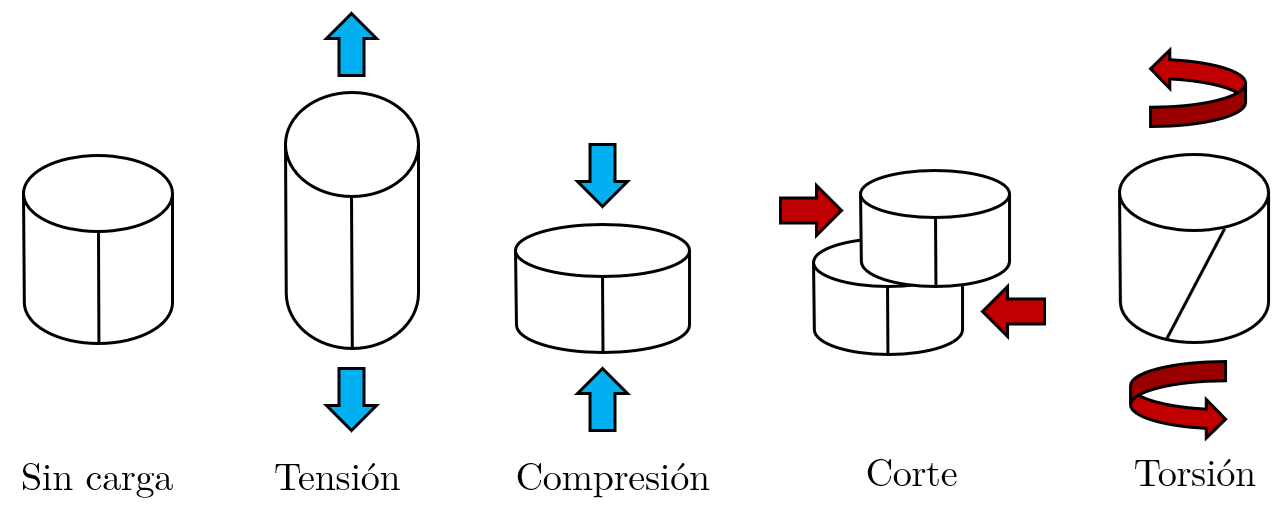
\includegraphics[width=0.9\linewidth]{imgs/cargas.png}
    \caption{Ejemplos de carga sobre un cilindro.}
    \label{fig:1}
\end{figure}

\begin{figure}[h!]
	\centering
	
\includegraphics[width=0.7\linewidth]{imgs/apoios.png}
	\caption{Ejemplos de condiciones de apoyo para una viga.}
	\label{fig:2}
\end{figure}

\subsection{Deformación}

Entenderemos como deformación al cambio geométrico de un cuerpo. Una forma de categorizar los tipos de deformación es respecto a la permanencia del cambio, donde si es reversible (al dejar de aplicar la carga), se le llama \textbf{deformación elástica}, y en caso contrario, \textbf{deformación plástica}. La parte elástica es resultado de interacciones atómicas y/o moleculares (atracción, repulsión, desenrrollamiento de cadenas) con la fuerza aplicada, mientras que lo plástico está relacionado con el desplazamiento permanente de átomos o moléculas en la estructura. Por lo anterior, siempre existe deformación elástica antes de que se dé deformación plástica a medida que incrementa el esfuerzo.

En el caso de la deformación elástica, esta se suele modelar como una relación entre átomos contiguos mediante resortes a través de la Ley de Hooke. La fuerza correspondería entonces a:

\begin{equation}
    F=k\Delta l \mathrm{[N]}
\end{equation}

Donde $k$ es la constante elástica y $\Delta l$ el cambio de longitud respecto al largo inicial o natural $l_{0}$. En el caso de los materiales, esta ley se puede extender de manera simplista como:

\begin{equation}
    \sigma=E\varepsilon \mathrm{[Pa]}
\end{equation}

Donde $E$ es el \textbf{módulo de Young} o de elasticidad del material y $\varepsilon$ a la deformación (adimensional). De esta manera, un material con mayor $E$ será más \textbf{rígido}, es decir, con menor tendencia a deformarse. Una forma de representar la deformación $\varepsilon$ \textit{nominal} es la siguiente:

\begin{equation}
    \varepsilon = \frac{\Delta l}{l_{0}}=\frac{l_{f}-l_{0}}{l_{0}}
\end{equation}

Lo anterior es una aproximación lineal muy conveniente y que se sostiene en varios casos, sin embargo el comportamiento real de los materiales puede variar significativamente del régimen lineal. Para estos casos existen modelos más complejos con dependencias multivariable. Los modelos para la deformación plástica tampoco son sencillos y quedan fuera del alcance de este apunte.

Las ecuaciones mostradas describen el caso ideal de deformación unidimensional, en el que un sólido se deforma exclusivamente a lo largo de un eje. La conservación de volumen implica que toda elongación longitudinal vaya acompañada de una contracción transversal (y viceversa), de modo que al estirar el material éste se estrecha en las direcciones perpendiculares. El \textbf{coeficiente de Poisson} $\nu$ cuantifica precisamente esta relación entre deformaciones longitudinal y transversal (adimensional). Sin embargo, ciertos materiales conocidos como \textbf{auxéticos} presentan un comportamiento opuesto: al someterse a tracción, también ensanchan su sección transversal, lo que se traduce en un valor negativo de $\nu$.

\subsection{Ensayo de tracción}

Una forma de caracterizar la relación esfuerzo-deformación es mediante el ensayo de tracción, como se observa en la Figura \ref{fig:2}. Como indica el nombre, una muestra de material con forma determinada es traccionado hasta la fractura, midiendo la fuerza y el desplazamiento de las mordazas que ejercen la fuerza, con cierto ajuste, o directamente a través de un extensómetro. Estos datos luego son transformados a su equivalente en esfuerzo y deformación, logrando las curvas observadas. 

\begin{figure}[h!]
    \centering
    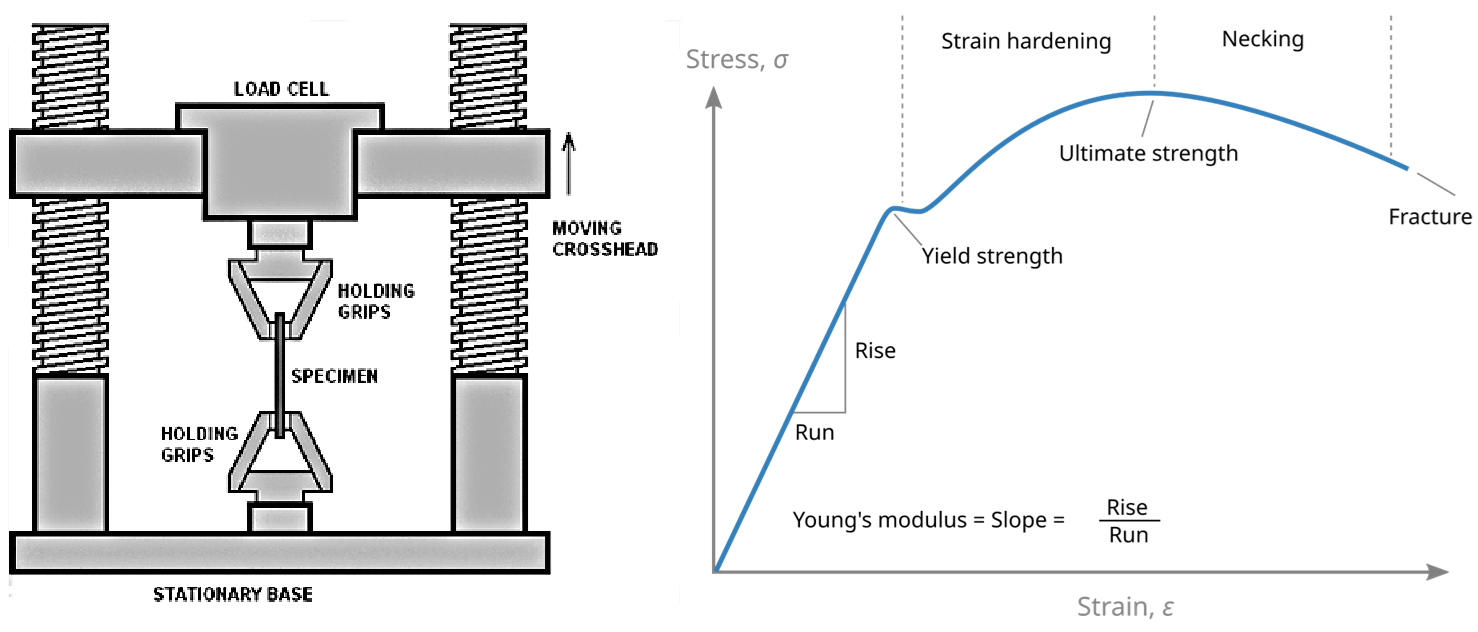
\includegraphics[width=0.97\linewidth]{imgs/es1.png}
    \caption{Ensayo de tracción, a la izquierda, diagrama de montaje, a la derecha, curva de esfuerzo-deformación típica de un metal dúctil.}
    \label{fig:2}
\end{figure}

Para el material exhibido en la Figura \ref{fig:2}, se observa una región inicial lineal, la cual corresponderá a la parte elástica. Al límite de esta región se le conoce como \textbf{esfuerzo de fluencia} o límite elástico (yield strength), simbolizado como $\sigma_{y}$, y es una \textbf{propiedad mecánica} de los materiales. La pendiente es entonces el módulo de Young $E$.

De la misma manera, al esfuerzo máximo en la curva le llamaremos \textbf{resistencia última a la tracción} $\sigma_{UTS}$ (ultimate strength). Más allá de este punto, se da un modo de deformación local conocido como \textbf{estrangulamiento} o \textit{necking} hasta la fractura del espécimen. Si bien, se observa que el esfuerzo baja en la curva, esto es así porque para el cálculo se considera el área inicial $A_{0}$ en lugar de la real. Con tal corrección, se observaría que el esfuerzo sigue aumentando.

La forma de esta curva no es igual para cada tipo de material, y también existen variaciones dentro de las mismas familias. En la Figura \ref{fig:3} se observan curvas representativas de cada tipo de material. De aquí se podría inferir, por ejemplo que en general los cerámicos son los materiales más rígidos y presentan un comportamiento elástico bastante lineal, mientras que los polímeros serían los menos resistentes. Entraremos en detalle respecto a los valores y comparaciones entre materiales en los próximos capítulos.

\begin{figure}[h!]
    \centering
    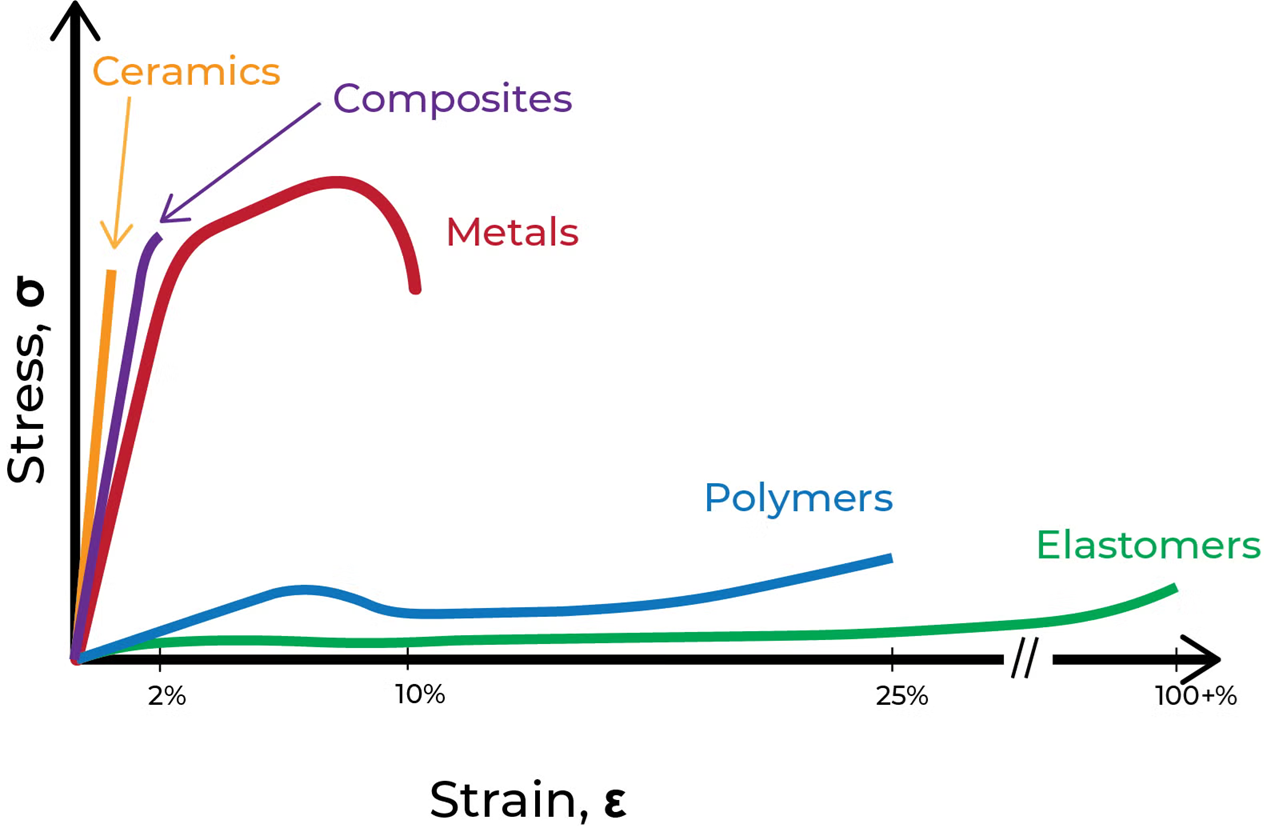
\includegraphics[width=0.85\linewidth]{imgs/tract.png}
    \caption{Formas típicas de las curvas esfuerzo-deformación para distintos tipos de materiales.}
    \label{fig:3}
\end{figure}

La \textbf{elongación final} $\varepsilon_{f}$ es la deformación alcanzada por la muestra hasta la falla. Es una propiedad mecánica que da cuenta de la ductilidad del material.

\section{Falla de componentes}

Como se mencionó anteriormente, a través del cálculo del estado de esfuerzos y diferentes métricas se podrá ajustar correctamente el diseño y la selección de materiales para prevenir fallas. Por ejemplo, si la deformación elástica es admisible, pero no así la plástica, un criterio sería simplemente:

\begin{equation}
    \sigma < \sigma_{y}
\end{equation}

Luego, se buscará un material con un $\sigma_{y}$ adecuado tal que cumpla la relación, o bien, se harán modificaciones en el diseño para disminuir el esfuerzo resultante. 

Considerando que estos modelos físicos surgen de aproximaciones y simplificaciones a la realidad, existe incerteza respecto a la exactitud de estos cálculos, por esto, se suele utilizar un \textbf{factor de seguridad} $f_{s}>1$ para garantizar seguridad en el servicio del componente, de la forma:

\begin{equation}
   \frac{\sigma_{y}}{\sigma} = f_{s}>1.0
\end{equation}

Esto aumenta la solicitud al material. La magnitud de este factor dependerá de normas y de la certeza en los cálculos empleados, intentando mantener el valor lo más reducido posible, pues su consecuencia podría implicar un sobredimensionamiento costoso del componente o sistema.

Una restricción sobre el diseño que podría ser más fuerte es limitar la deformación. Para aplicaciones de precisión o de tolerancias ajustadas, una deformación pequeña puede generar contactos indeseados entre componentes o modificar la trayectoria de otros.

Los criterios ejemplificados anteriormente son estáticos, es decir, no consideran fenómenos asociados al daño acumulado con el avance del tiempo.

Una de estas formas de daño acumulado es la \textbf{fatiga}, y está relacionada con el crecimiento de grietas o defectos en la estructura del material hasta generar una fractura (Figura \ref{crack}). Una \textbf{grieta} es una discontinuidad que no permite la distribución uniforme del esfuerzo, sino que lo concentra en su reducida geometría local, fracturando secuencialmente el material.

\begin{figure}[h!]
    \centering
    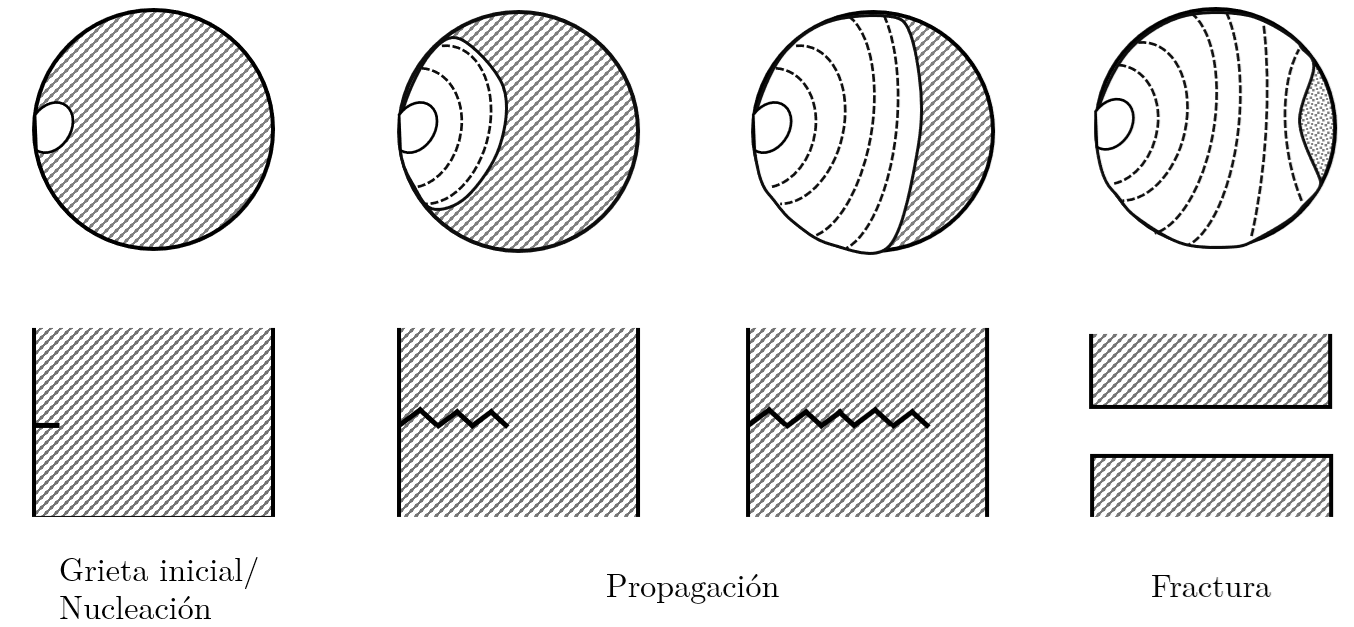
\includegraphics[width=0.9\linewidth]{imgs/crack.png}
    \caption{Mecanismo de crecimiento de grieta por fatiga. (1) Nucleación o iniciación, (2) Propagación, (3) Fractura. El avance de la grieta deja una superficie estriada, hasta la falla frágil súbita, donde la superficie queda con aspecto rugoso.}
    \label{crack}
\end{figure}

Este crecimiento de grieta a través de la fatiga está relacionado con \textbf{cargas cíclicas} y debilita al material, reduciendo su vida útil a pesar de que los esfuerzos no sean superiores a $\sigma_{y}$. El origen, velocidad y daño inducido por estas cargas depende de múltiples variables, por ejemplo:

\begin{itemize}
    \item Propiedades intrínsecas del material.
    \item Carga: Tipo, amplitud, media, y en menor medida, frecuencia.
    \item Geometría: Tamaño de la pieza, concentradores de esfuerzo, defectos.
    \item Calidad de la superficie: Tratamiento, grietas.
    \item Condiciones ambientales: Humedad, temperatura, agentes químicos.
\end{itemize}

La fatiga como parámetro de diseño permite calcular la \textbf{vida útil} del material, mediante el uso de la curva de vida amplitud-ciclos o diagrama de Wöhler (Figura \ref{fig:4}).

\begin{figure}[h!]
    \centering
    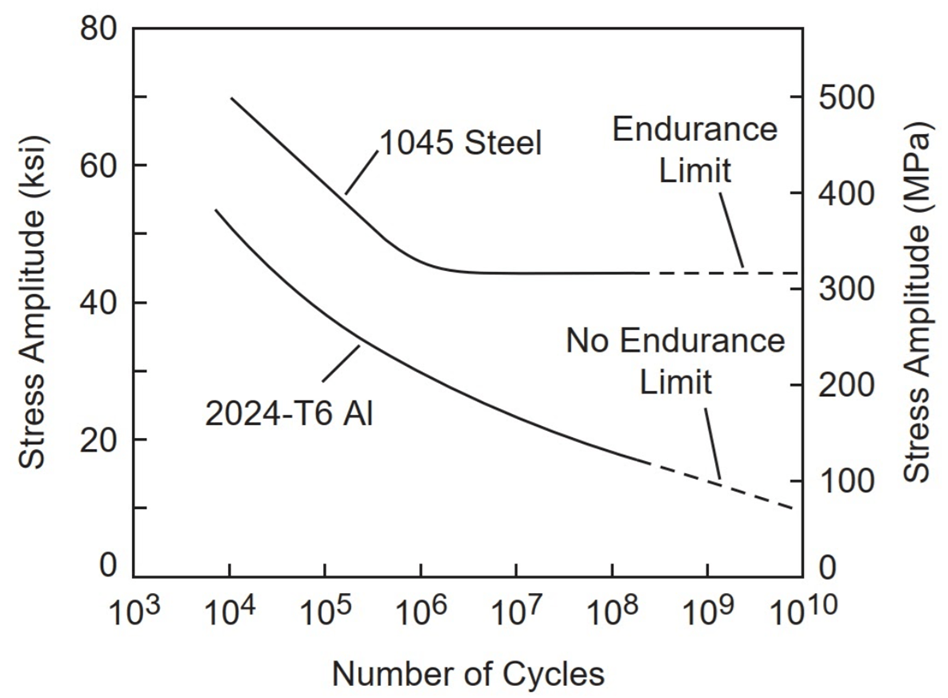
\includegraphics[width=0.65\linewidth]{imgs/sn.png}
    \caption{Curva de Wöhler para aleación de aluminio y acero.  \href{https://sdcverifier.com/structural-engineering-101/fatigue-strength-and-limit-understanding-materials-specific-data/}{Fuente}}
    \label{fig:4}
\end{figure}

En el ejemplo se observan 2 aleaciones metálicas ampliamente estudiadas. Nótese el \textit{endurance limit} (límite de fatiga, frecuentemente simbolizado como $\sigma_{ew}$), el cual indica que para amplitudes inferiores a este el material tiene vida infinita.

Dado que esto depende en parte de un tamaño de grieta, el material también podría fallar de manera estática si es que posee una grieta inicial. Esta grieta avanzaría de forma rápida e inestable hasta la ruptura, sin necesidad de ciclos de carga en función de la \textbf{resistencia a la propagación de grietas} del material.

El parámetro $K_{IC}$, determinado mediante ensayos cuantifica la resistencia intrínseca del material al crecimiento de grietas (bajo ciertas condiciones específicas, como régimen elástico) y resulta fundamental para diseñar y evaluar componentes con concentradores de esfuerzo, pues define el umbral crítico que evita fallas frágiles. Una forma de usar este parámetro es comparándolo con el \textbf{factor de intensidad de la grieta} $K$ $(\mathrm{[Mpa\sqrt{m}]})$: 

\begin{equation}
    K=\beta \sigma\sqrt{a\pi} < K_{IC} \implies \text{No hay fractura rápida}
\end{equation}

Con $\beta$ un parámetro geométrico y $a$ el tamaño de la grieta. Si bien, esta medida podría dar cuenta de la \textbf{tenacidad} del material, la energía absorbida antes de la fractura (Figura \ref{fig:5}, área bajo las curvas), existen otros ensayos y medidas más directas que consideran además la deformación plástica, como el ensayo de impacto de Charpy o Izod. Los materiales frágiles suelen presentar deformación plástica despreciable (como se observa en la Figura \ref{fig:5}) y alta sensibilidad a concentradores de esfuerzo, como sucede con vidrios y cerámicos.

\begin{figure}[h!]
    \centering
    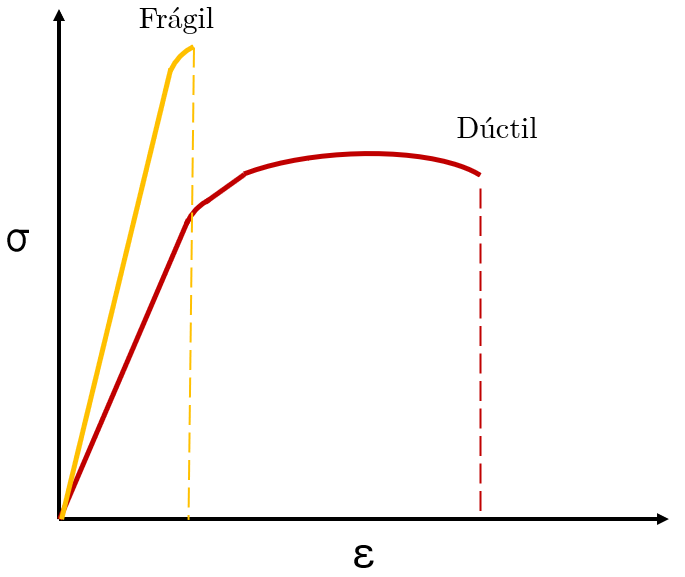
\includegraphics[width=0.5\linewidth]{imgs/tough.png}
    \caption{Curva de esfuerzo deformación para un material dúctil (alta deformación plástica) y uno frágil. La tenacidad correspondería a la energía absorbida antes de la fractura, representada por el área bajo cada curva.}
    \label{fig:5}
\end{figure}

Otra causa para la falla de materiales es la \textbf{termofluencia} o \textbf{creep}, que corresponde a deformación progresiva y dependiente del tiempo que sufre un material bajo carga constante a temperaturas elevadas, que puede culminar en falla sin necesidad de aumentar la tensión aplicada. 

\section{Dureza}

La dureza es una propiedad mecánica de los materiales que mide la capacidad de resistir la penetración o \textbf{deformación plástica localizada en su superficie} bajo una carga concentrada (Figura \ref{dur}). Se determina mediante ensayos de indentación (Brinell, Rockwell, Vickers, Shore, entre otros) que cuantifican el tamaño de la huella dejada por un indentador bajo una carga controlada. Como propiedad mecánica complementaria a la resistencia a la tracción, la dureza ofrece una medida rápida y casi no destructiva de la \textbf{resistencia al desgaste y a la abrasión}.

\begin{figure}[h!]
    \centering
    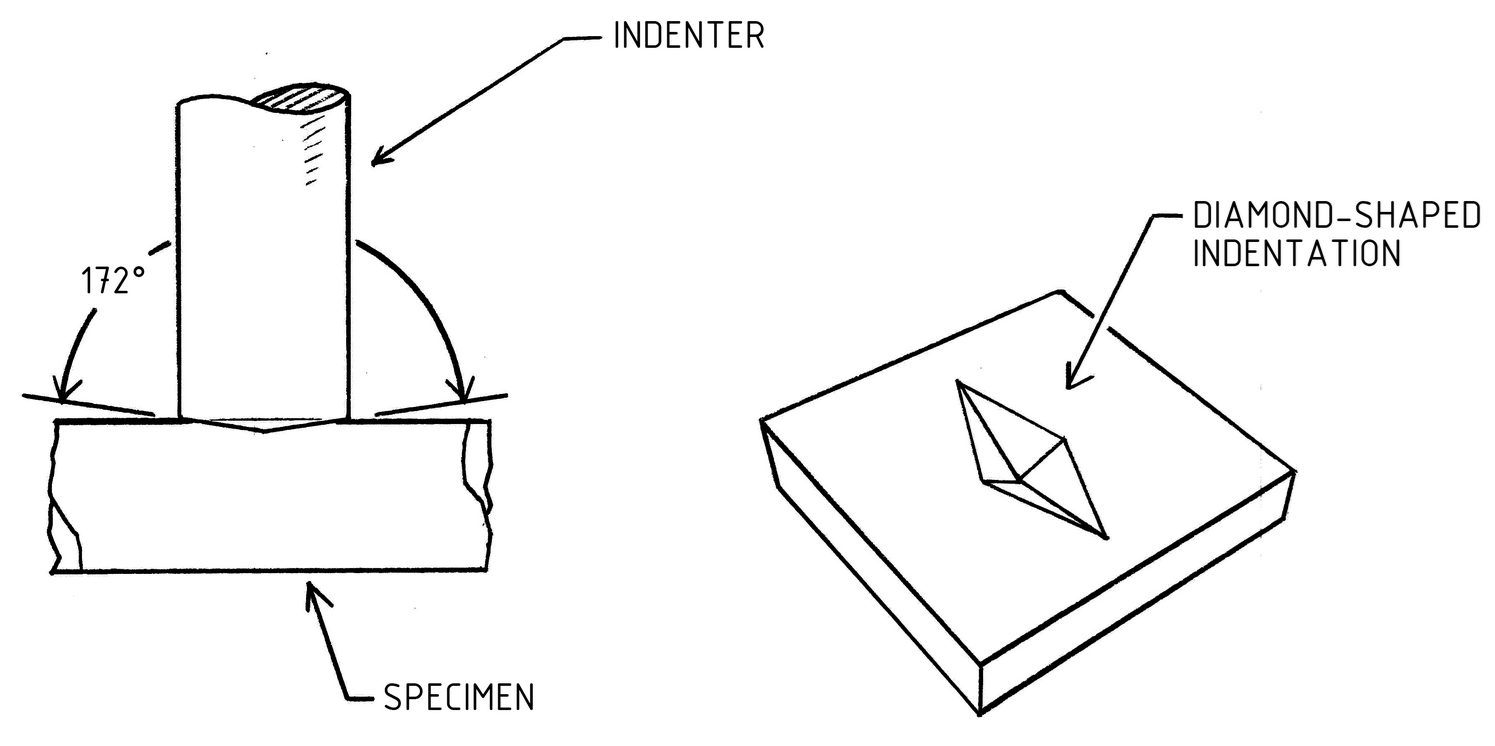
\includegraphics[width=0.6\linewidth]{imgs/indent.png}
    \caption{Ensayo de dureza Brinell, indentador esférico.}
    \label{dur}
\end{figure}

Así, en la interacción mecánica entre dos materiales de diferente dureza, el más blando es más susceptible a deformarse y ceder, mientras que el más duro actúa como agente agresor y conserva su forma. Esta diferencia de dureza determinará el mecanismo de desgaste (abrasión, adhesión, fatiga de contacto) que primará en la interacción, así como la tasa de desgaste.

Un material de alta dureza evita la deformación plástica localizada y la concentración de tensiones que dan origen a grietas, prolongando la vida útil del componente. La superficie dura dificulta la penetración y el arranque de material bajo cargas de deslizamiento, reduciendo el desgaste por fricción, luego, estos materiales son ideales para soportar cargas deslizantes en transmisión o para aplicaciones con impactos frecuentes.

Por otro lado, un material frágil presenta baja tenacidad y prácticamente nula ductilidad, de modo que se fractura de forma repentina al superar su límite elástico. Esto conlleva fallos catastróficos sin señal previa, mala absorción de energía ante impactos o vibraciones y alta susceptibilidad a la propagación de grietas, lo que limita su uso en aplicaciones donde la seguridad y la fiabilidad sean críticas.

Dado que estos fenómenos se presentan principalmente en la superficie de un material, se han desarrollado técnicas o \textbf{tratamientos de endurecimiento superficial} que generan una capa externa de elevada dureza y resistencia al desgaste, mientras el núcleo conserva la ductilidad y tenacidad necesarias, optimizando así la durabilidad y seguridad de componentes.

\section{Transferencia de calor}

Se define la temperatura como una magnitud física intensiva, proporcional a la energía cinética media de las partículas que constituyen un sistema termodinámico. Cuando dos cuerpos a distinta temperatura entran en contacto, se genera un flujo de energía térmica entre ellos, denominado transferencia de calor, que persiste hasta alcanzar el equilibrio térmico. La transferencia de calor se da a través de 3 mecanismos (Figura \ref{calors}):

\begin{itemize}
  \item Conducción: transferencia de energía mediante colisiones entre partículas adyacentes en un material sólido o estacionario.
  \item Convección: transporte de calor por el movimiento de un fluido (líquido o gas), ya sea natural o forzado.
  \item Radiación: emisión y absorción de energía en forma de ondas electromagnéticas, que puede ocurrir incluso en el vacío.
\end{itemize}

Los fenómenos de transferencia térmica están determinados por las propiedades termofísicas de los materiales. Cuando un flujo de calor atraviesa un sólido, la variación de su temperatura viene definida por:

\begin{itemize}
  \item Densidad, $rho\,\mathrm{[kg/m^{3}]}$, masa por unidad de volumen.
  \item Calor específico, $c_p\,\mathrm{[J/(kg\,K)]}$, energía necesaria para elevar 1 K la temperatura de 1 kg.
  \item Conductividad térmica, $k\,\mathrm{[W/(mK)]}$, capacidad de transmitir el flujo de calor por unidad de gradiente de temperatura.
\end{itemize}

\begin{figure}[h!]
    \centering
    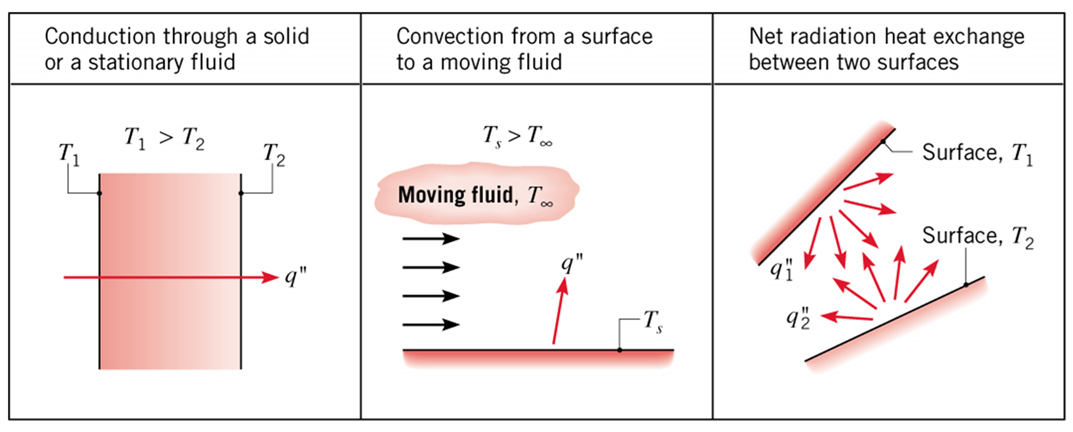
\includegraphics[width=0.9\linewidth]{imgs/calor.png}
    \caption{Mecanismos de transferencia de calor.\cite{incrop}}
    \label{calors}
\end{figure}

La difusividad térmica, \(\alpha\), sintetiza estas tres magnitudes y mide la rapidez con que se propaga una perturbación térmica:

\begin{equation}
  \alpha = \frac{k}{\rho\,c_p}
  \quad [\mathrm{m^2/s}]
\end{equation}

En la práctica todos los materiales exhiben alguna \textbf{dependencia de sus propiedades mecánicas con la temperatura}. No obstante, hay magnitudes que muestran variaciones muy pequeñas y a menudo se tratan como constantes en ciertas aplicaciones. En la Figura \ref{fig:ttt} se observa una variación leve del módulo de Young para dos aleaciones de acero en un rango amplio de temperaturas, mientras que el límite elástico presenta una variación más severa.

\begin{figure}[h!]
    \centering
    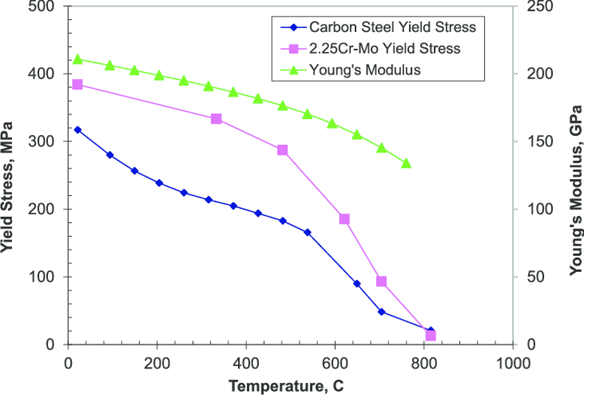
\includegraphics[width=0.7\linewidth]{imgs/tempgraf.png}
    \caption{Variación del módulo de Young y el límite elástico para dos aleaciones de acero.\cite{tempyoung}}
    \label{fig:ttt}
\end{figure}

Un fenómeno relevante ligado al cambio de temperatura es la \textbf{dilatación térmica} $\beta$. El aumento de la energía cinética de las partículas desplaza su distancia de equilibrio, alejándolas. Como consecuencia, el cuerpo presentará un aumento de volumen que dependerá del parámetro $\beta$, o reducción en caso de que la temperatura descienda.

La dilatación térmica en sistemas mecánicos puede alterar significativamente la holgura entre dos componentes. Si existe movimiento relativo, surgirán fuerzas de rozamiento y abrasión en caso de contacto; y si la expansión está impedida, se generan presiones internas que originan un \textbf{esfuerzo térmico}.

\section{Materiales de ingeniería}

\subsection{Clasificación}

Un material de ingeniería es aquel cuya composición y estructura se controlan deliberadamente durante su fabricación, siguiendo métodos y pruebas estandarizadas para que sus propiedades (mecánicas, térmicas, eléctricas o químicas) sean siempre las mismas (dentro de cierto rango). De esta forma, permiten diseñar piezas y estructuras con certeza respecto a su comportamiento y desempeño.

Estos materiales se suelen agrupar en 4 familias en función del \textbf{enlace químico} predominante en su estructura (Figura \ref{bons}), pues esto determinará en gran medida las propiedades mecánicas, térmicas y eléctricas:

\begin{figure}[h!]
    \centering
    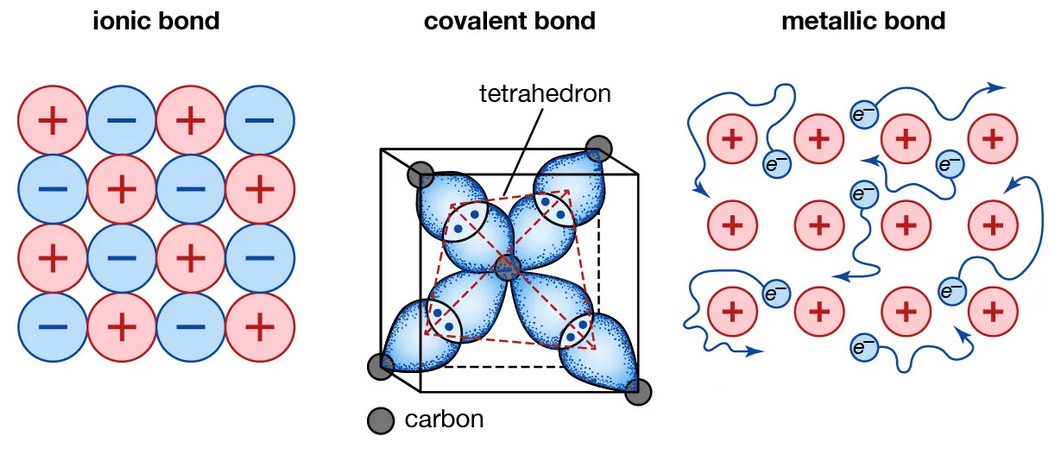
\includegraphics[width=1.0\linewidth]{imgs/bonds.png}
    \caption{Tipos de enlaces atómicos en materiales de ingeniería.} 
    \label{bons}
\end{figure}

\textbf{Materiales metálicos}
    \begin{itemize}
      \item Enlace metálico con electrones libres.
      \item Alta conductividad térmica y eléctrica.
      \item Excelente ductilidad, maleabilidad y tenacidad.
      \item Buena resistencia mecánica y capacidad de deformación plástica.
    \end{itemize}

\textbf{Materiales cerámicos}
  
    \begin{itemize}
      \item Enlaces iónicos y/o covalentes muy fuertes.
      \item Elevada dureza y estabilidad a altas temperaturas.
      \item Baja tenacidad: comportamiento frágil ante impactos.
      \item Aislantes eléctricos y térmicos.
    \end{itemize}

\textbf{Materiales poliméricos}
  
    \begin{itemize}
      \item Cadenas moleculares unidas por enlaces covalentes.
      \item Baja densidad y buen aislamiento térmico y eléctrico.
      \item Amplia variedad de rigidez y elasticidad (termoplásticos, termofijos, elastómeros).
      \item Resistencia química y facilidad de procesado.
    \end{itemize}

\textbf{Materiales compuestos}
  
    \begin{itemize}
      \item Matriz (polímero, metal o cerámico) reforzada con fibras o partículas.
      \item Elevada resistencia específica (resistencia normalizada por la masa).
      \item Propiedades a medida según combinación de componentes.
      \item Versatilidad en forma y aplicación, adaptables a exigencias de diseño.
    \end{itemize}

Esta clasificación y las propiedades comunes de cada familia simplifican la selección inicial de materiales para las condiciones operativas. Sin embargo, los \textbf{parámetros de diseño} (restricciones y objetivos que guían el proceso) determinan la idoneidad final de la elección. Por ejemplo, si se necesita una pieza rígida y resistente a la corrosión, un cerámico podría parecer la opción ideal; no obstante, podría resultar incompatible con los procesos de manufactura habituales o disponibles. De esta manera, la selección del material va a seguir los siguientes criterios:

\begin{itemize}
    \item Rendimiento mecánico (resistencia, dureza, tenacidad).
    \item Condiciones de servicio (temperatura, ambiente químico, cargas cíclicas).
    \item Factores económicos (coste de materia prima, procesamiento y reciclado).
    \item  Sostenibilidad y ciclo de vida (reutilización, huella ambiental).
    \item Disponibilidad y normativas (certificaciones, estandarización internacional).
\end{itemize}

Dada la composición química y el tipo de enlace, el material adquiere una \textbf{microestructura} que describe cómo se agrupan sus átomos. Si ese agrupamiento presenta un orden periódico a largo alcance, hablamos de una \textbf{red cristalina}; en caso contrario, la estructura es \textbf{amorfa} (Figura \ref{cris}), y semicristalino cuando presenta sectores organizados. En un sólido cristalino, esos arreglos atómicos ordenados se extienden más allá de la escala atómica para formar \textbf{granos} distinguibles (Figura \ref{mic}), dentro de los cuales todos los cristales comparten una misma orientación. Esta organización, sea en forma de granos o de red desordenada, condiciona de manera decisiva las propiedades mecánicas, térmicas y eléctricas del material.

\begin{figure}[h!]
    \centering
    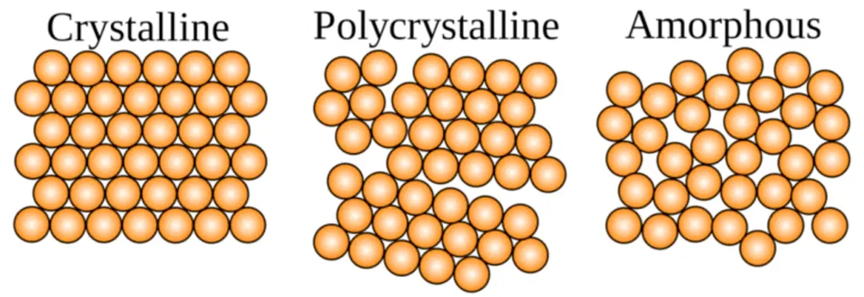
\includegraphics[width=0.9\linewidth]{imgs/crist.png}
    \caption{Esquema de microestructuras: Cristalina, semicristalina y amorfa.}
    \label{cris}
\end{figure}

La microestructura del material puede variar en cada etapa del ciclo de vida: durante su formación inicial, en el procesamiento de la materia prima, a través de tratamientos posteriores y durante el servicio. Al ajustar las diferentes variables, podemos diseñar arreglos atómicos y granulometrías que optimicen las propiedades finales del material para algún objetivo específico. Eventualmente, durante el uso, las condiciones podrían modificar o dañar la microestructura del material, iniciando mecanismos de falla.

\begin{figure}[h!]
    \centering
    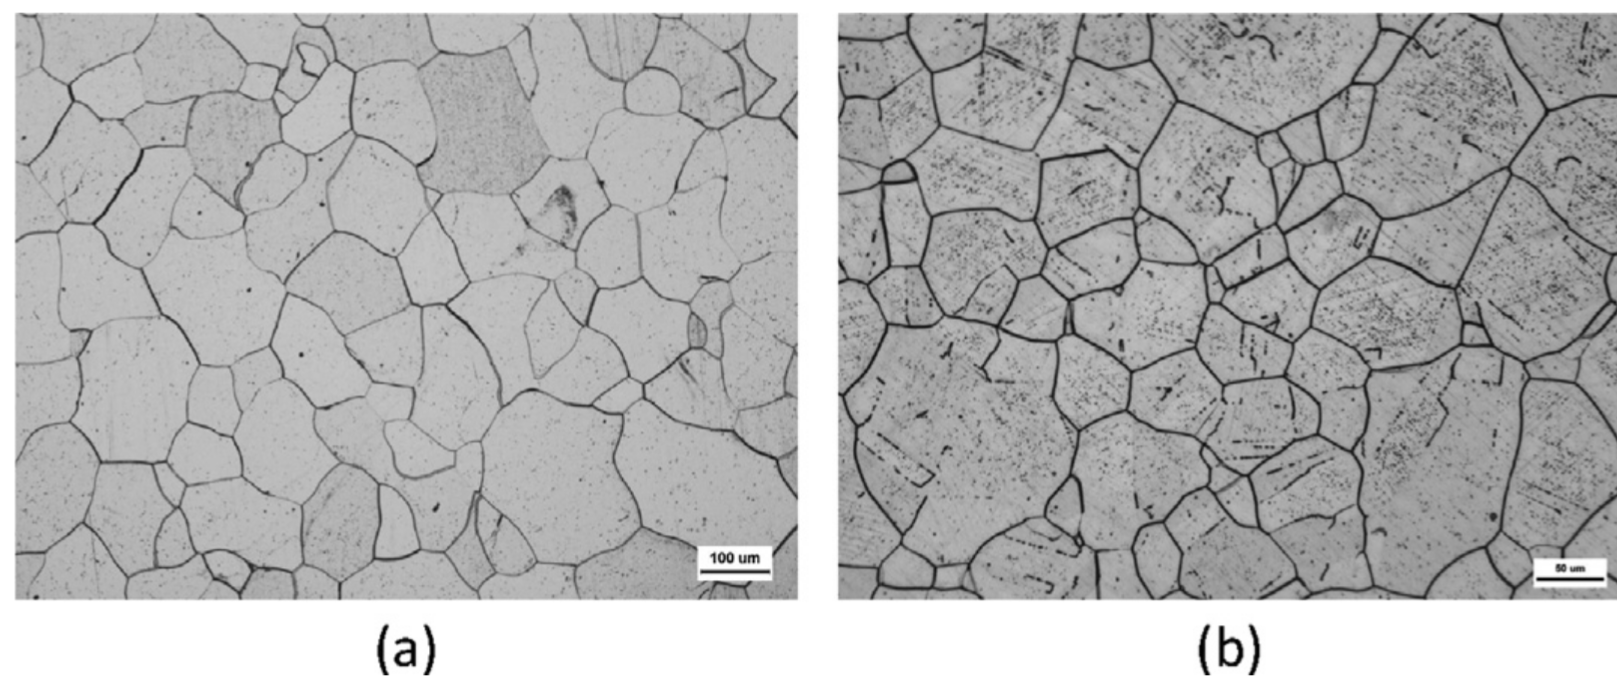
\includegraphics[width=1.0\linewidth]{imgs/micr.png}
    \caption{Fotografía de granos en un material a través de microscopio. a) Granos de ferrita en hierro de alta pureza, b) Granos de austenita en acero inoxidable.\cite{acers}}
    \label{mic}
\end{figure}

\subsection{Materiales y valores típicos}

Como vimos anteriormente, las distintas familias de materiales exhiben rangos característicos de propiedades, pero la elección de un material implica evaluar múltiples criterios de diseño. Para simplificar este proceso, resulta muy útil representar gráficamente las variables clave. En la Figura \ref{props}, por ejemplo, los materiales se sitúan según su rigidez y densidad en un diagrama de Ashby; así, al fijar una rigidez objetivo, podemos identificar de inmediato la opción más ligera que la cumpla.

\begin{figure}[h!]
    \centering
    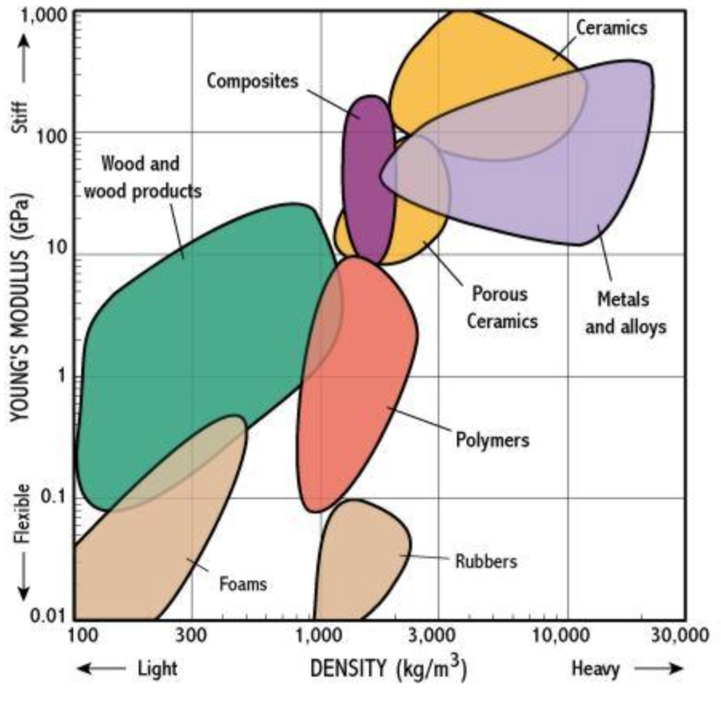
\includegraphics[width=0.6\linewidth]{imgs/comp.png}
    \caption{Diagrama de Ashby de rigidez-densidad para materiales de ingeniería, útil para optimizar la resistencia a la deformación/peso. \href{http://www-materials.eng.cam.ac.uk/mpsite/interactive_charts/}{Fuente}}
    \label{props}
\end{figure}

Actualmente, este tipo de mapas se da en aplicaciones computacionales interactivas, las cuales permiten hacer el cruce de parámetros y agilizar la selección del material, así como otorgar información relevante respecto a los costos, aplicaciones típicas, procesos de conformado, etc. De esta manera, la labor de ingeniería no es solo identificar el material que cumple con las exigencias mecánicas, sino que además optimizar el desempeño, la economía y la sostenibilidad del diseño en estudio.

En la formación de ingeniería mecánica y metalúrgica se presta especial atención a los materiales de uso industrial más extendido. El acero ocupa un lugar central: una \textbf{aleación} (mezcla de elementos en la que al menos uno es metálico) de hierro y carbono. Las variaciones en su composición (contenido de carbono y elementos de aleación) y en los \textbf{procesos de fabricación} (laminado, forja, extrusión, tratamientos térmicos) definen la microestructura resultante y, con ello, sus propiedades mecánicas. Otras aleaciones estudiadas son las de aluminio (aluminio combinado con cobre), bronce (cobre y estaño), y latón (cobre y zinc).

\begin{table}[htbp]
  \centering
  \small
  \caption{Composición y costo de familias de materiales}
  \label{tab:prop_mat_comp_costo}
  \begin{tabular}{@{} l l c @{}}
    \toprule
    Material                  & Composición                          & Costo (\$/kg) \\
    \midrule
    Aceros al carbono         & Fe + 0.05–1.2\% C                    & 0.8–1.2       \\
    Aceros de aleación        & Fe + C + 2–8\% (Cr, Ni, Mo, V…)      & 1.0–1.5       \\
    Aleaciones de aluminio    & Al + (Si, Mg, Cu, Zn)                & 1.5–3.0       \\
    Aleaciones de titanio     & Ti + (Al, V)                         & 20–30         \\
    Superaleaciones de níquel & Ni + Cr, Co, Al, Ti…                 & 50–80         \\
    Cobre puro                & Cu                                   & 5.0–7.0       \\
    Bronce                    & Cu + 5–12\% Sn                       & 6.0–10.0      \\
    Latón                     & Cu + 30–40\% Zn                      & 4.0–6.0       \\
    Vidrios                   & SiO$_2$, Na$_2$O, CaO…               & 0.3–1.0       \\
    Polímeros termoplásticos  & C, H, O (PE, PP, ABS…)               & 1.0–3.0       \\
    Polímeros termoestables   & C, H, O, N (epóxicos, fenólicos…)    & 2.0–4.0       \\
    Elastómeros               & C, H, O (EPDM, NBR, silicona…)       & 1.0–5.0       \\
    Fibra de vidrio           & Filamentos de vidrio en matriz polim. & 2–5           \\
    Fibra de carbono          & Filamentos de carbono en matriz polim. & 15–50         \\
    Cerámicos (óxidos)        & Al$_2$O$_3$, ZrO$_2$                 & 3.0–6.0       \\
    Cerámicos (carburos)      & SiC, WC                              & 30–50         \\
    Madera dura               & Celulosa, lignina                    & 0.5–1.0       \\
    \bottomrule
  \end{tabular}
\end{table}

\begin{table}[htbp]
  \centering
  \small
  \caption{Propiedades mecánicas de familias de materiales}
  \label{tab:prop_mat_mecanicas}
  \begin{tabular}{@{} l c c c c @{}}
    \toprule
    Material                  & $E$ (GPa) & $\sigma_y$ (MPa) & Dureza (HV/Shore) & $\sigma_UTS$ (MPa)\tnote{1} \\
    \midrule
    Aceros al carbono         & 190–210   & 250–800          & 150–450 HV        & 400–1200          \\
    Aceros de aleación        & 190–210   & 300–1000         & 200–600 HV        & 500–1400          \\
    Aleaciones de aluminio    & 65–80     & 50–500           & 25–150 HV         & 90–600            \\
    Aleaciones de titanio     & 100–120   & 450–1000         & 200–400 HV        & 550–1200          \\
    Superaleaciones de níquel & 210–240   & 700–1200         & 250–550 HV        & 900–1500          \\
    Cobre puro                & 110–130   & 50–300           & 40–120 HV         & 200–500           \\
    Bronce                    & 100–120   & 200–400          & 60–200 HV         & 300–550           \\
    Latón                     & 90–110    & 150–350          & 55–200 HV         & 300–500           \\
    Vidrios                   & 60–90     & —                & 500–700 HV        & 30–100¹           \\
    Polímeros termoplásticos  & 1–5       & 20–100           & 30–100 Shore D    & 40–100            \\
    Polímeros termoestables   & 2–10      & 30–80            & 70–120 Shore D    & 50–120            \\
    Elastómeros               & 0.01–0.1  & 5–30             & 30–90 Shore A     & 5–30              \\
    Fibra de vidrio           & 20–40     & 150–350          & 70–95 Shore D     & 150–500           \\
    Fibra de carbono          & 70–250    & 600–2000         & 70–95 Shore D     & 800–2500          \\
    Cerámicos (óxidos)        & 200–400   & —                & 1000–1500 HV      & 200–500¹          \\
    Cerámicos (carburos)      & 350–450   & —                & 2000–3000 HV      & 400–1000¹         \\
    Madera dura               & 10–16     & 40–100           & 20–60 Janka       & 80–150            \\
    \bottomrule
  \end{tabular}

  \vspace{1mm}
  \footnotesize
  — propiedad no aplicable; ¹ resistencia a flexión en lugar de UTS.
\end{table}

\newpage

\begin{table}[htbp]
  \centering
  \small
  \caption{Densidad, conductividad térmica y coeficiente de dilatación de familias de materiales}
  \label{tab:prop_mat_fisicas_sin_costo}
  \begin{tabular}{@{} l c c c @{}}
    \toprule
    Material                  & $\rho\, \mathrm{(g/cm^{3})}$ & $k$ (W/(mK)) & $\alpha\,\mathrm{(10^{-6}/K)}$ \\
    \midrule
    Aceros al carbono         & 7.7–8.1           & 45–60               & 10–13                  \\
    Aceros de aleación        & 7.7–8.1           & 40–60               & 10–14                  \\
    Aleaciones de aluminio    & 2.6–2.8           & 120–180             & 22–25                  \\
    Aleaciones de titanio     & 4.4–4.6           & 6–15                & 8–10                   \\
    Superaleaciones de níquel & 8.1–8.3           & 8–15                & 12–16                  \\
    Cobre puro                & 8.9–9.0           & 380–400             & 16–17                  \\
    Bronce                    & 8.7–8.9           & 40–55               & 17–18                  \\
    Latón                     & 8.4–8.7           & 100–125             & 19–20                  \\
    Vidrios                   & 2.4–2.6           & 0.8–1.4             & 8–9                    \\
    Polímeros termoplásticos  & 0.9–1.5           & 0.1–0.5             & 50–200                 \\
    Polímeros termoestables   & 1.1–1.4           & 0.2–0.3             & 30–100                 \\
    Elastómeros               & 0.8–1.4           & 0.15–0.3            & 70–300                 \\
    Fibra de vidrio           & 1.8–2.0           & 0.3–0.5             & 10–15                  \\
    Fibra de carbono          & 1.5–1.6           & 5–10                & 0–1                    \\
    Cerámicos (óxidos)        & 3.8–4.1           & 20–40               & 5–8                    \\
    Cerámicos (carburos)      & 3.1–3.2           & 80–120              & 3–5                    \\
    Madera dura               & 0.6–0.85          & 0.15–0.25           & 3–5                    \\
    \bottomrule
  \end{tabular}
\end{table}

\subsection{Polímeros}

Los polímeros son macromoléculas formadas por la \textbf{repetición de unidades básicas} (monómeros) unidas mediante enlaces covalentes. Están constituidos principalmente por átomos de carbono e hidrógeno, y en ocasiones incorporan oxígeno, nitrógeno, azufre o silicio. Según su comportamiento térmico y la estructura de sus cadenas, se clasifican en (Figura \ref{plmrs}):

\begin{itemize}
  \item \textbf{Termoplásticos}: polímeros lineales o ligeramente ramificados que al calentarse ablandan o funden y, al enfriarse, recuperan su rigidez. Este fenómeno es reversible y permite múltiples ciclos de conformado. Ejemplos: polietileno (PE), polipropileno (PP), policloruro de vinilo (PVC).
  \item \textbf{Termoestables}: resinas que, mediante un proceso de curado o reticulación, forman una red tridimensional de enlaces cruzados. Esta estructura impide que el material vuelva a fundirse tras el calentamiento, garantizando rigidez y resistencia térmica. Ejemplos: resinas epoxi, fenol-formaldehído, poliéster insaturado.
\end{itemize}

Un caso particular en los polímeros es el de los elastómeros, los cuales poseen macromoléculas en una red desordenada y móvil, con una baja densidad de enlaces entrecruzados. Los entrecruzamientos actúan como puntos de anclaje que fijan la longitud máxima de cada cadena, evitando el flujo plástico, pero al mismo tiempo permiten el desenredo y replegado elástico de segmentos bajo tensión. Dependiendo del tipo de enlace entrecruzado, un elastómero puede ser termoplástico (enlace débil) o termoestable (enlace covalente).

La síntesis de polímeros suele iniciarse en fase líquida, en disolución, suspensión o masa fundida, donde los monómeros reaccionan por adición o condensación para generar oligómeros de bajo peso molecular. A medida que avanza la reacción y aumentan la longitud y, en el caso de los termoestables, la densidad de enlaces cruzados, la mezcla evoluciona de un estado fluido o viscoso hacia un estado semisólido y, finalmente, sólido. Este comportamiento se ilustra en el Cuadro \ref{tab:etapas_polimeros}.

\begin{figure}[h!]
    \centering
    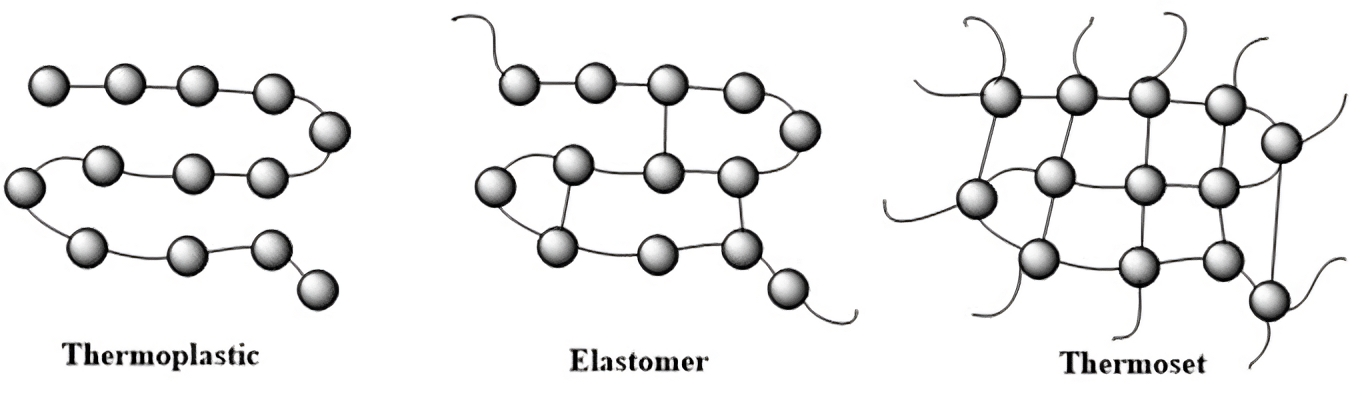
\includegraphics[width=1.0\linewidth]{imgs/elastomer.png}
    \caption{Estructura molecular en distintos tipos de polímeros.}
    \label{plmrs}
\end{figure}

\begin{table}[h]
  \centering
  \caption{Etapas generales en la producción de polímeros}
  \label{tab:etapas_polimeros}
  \begin{tabular}{|P{2.5cm}|P{3.5cm}|P{4cm}|P{4.5cm}|}
    \hline
    \textbf{Etapa}            & \textbf{Estado de la mezcla}        & \textbf{Termoplásticos}                                                    & \textbf{Termoestables}                                                        \\ \hline
    Monómeros                 & Líquido o gas                       & Monómeros aislados listos para reaccionar                                   & Monómeros o precursores con múltiples sitios reactivos                         \\ \hline
    Pre polimerización         & Viscosa (oligómeros cortos)         & Formación de cadenas lineales o ramificadas de bajo peso molecular & Formación de resinas líquidas o prepolímeros con grupos funcionales reactivos   \\ \hline
    Polimerización            & Semifundida o fundida               & Crecimiento de cadenas por adición o condensación sin enlaces cruzados       & Reacción simultánea de formación de cadena y reticulación progresiva            \\ \hline
    Moldeo y conformado       & Fundido (\,TP\,), líquido (\,TE\,)  & Moldeo, enfriado y ciclo repetible tras nueva fusión                         & Moldeo inicial (inyección, compresión) seguido de curado irreversible          \\ \hline
    Post-tratamiento y curado & Sólido                              & Opcional: orientación, recocido, mejora de propiedades                      & Curado final para completar la red tridimensional y obtener rigidez permanente  \\ \hline
  \end{tabular}
\end{table}

En ingeniería, aunque los polímeros suelen exhibir una resistencia mecánica inferior a la de metales o cerámicas, compensan esa desventaja con un coste reducido, una gran versatilidad en los procesos de conformado y una elevada resistencia a la corrosión y a agentes químicos.

Los polímeros muestran una marcada dependencia de la temperatura, lo cual puede limitar su rango de servicio pero al mismo tiempo facilita enormemente su conformado (moldeo, extrusión, inyección). Esta sensibilidad térmica se traduce en variaciones drásticas del módulo de elasticidad y acota los rangos operativos prácticos. 

El fenómeno principal que rige el comportamiento mecánico de los polímeros a bajas y medias temperaturas es la \textbf{transición vítrea} (Figura \ref{vitr}). Se trata de un cambio abrupto en la rigidez y en las propiedades viscoelásticas cuando se supera la \textbf{temperatura de transición vítrea} (\(T_{g}\)). 

Por debajo de \(T_{g}\), las cadenas poliméricas están \comillas{congeladas} en un estado rígido y frágil, con muy escasa movilidad. Al pasar por \(T_{g}\), se activan movimientos de rotación y traslación local de los segmentos de cadena, dando lugar a un estado gomoso o viscoelástico con mayor capacidad de deformación y absorción de energía. Esta transición se explica por el incremento de la energía térmica disponible para vencer las barreras conformacionales de los enlaces simples a lo largo de la macromolécula.

La \textbf{cristalinidad} de un polímero determina sus propiedades térmicas, mecánicas y ópticas. Según el grado de ordenamiento de las cadenas, se pueden distinguir dos grandes familias:

\begin{itemize}
  \item \textbf{Semicristalino:} combinan regiones cristalinas ordenadas (cristalitas) con zonas amorfas. Exhiben un punto de fusión (\(T_m\)) correspondiente a desorganización de las porciones cristalinas y un \(T_g\) asociado a las zonas amorfas. La presencia de cristalinidad aporta mayor rigidez, resistencia química y mejor barrera a gases. Ejemplos típicos: polietileno (PE), polipropileno (PP) y tereftalato de polietileno (PET).
  \item \textbf{Amorfo:} las cadenas carecen de orden a largo alcance y presentan únicamente una temperatura de transición vítrea (\(T_g\)). No existe un punto de fusión bien definido, por lo que mantienen transparencia y flexibilidad a temperatura ambiente. Ejemplos típicos: poliestireno (PS), poli(metacrilato de metilo) (PMMA) y policarbonato (PC).
\end{itemize}

\begin{figure}[h!]
    \centering
    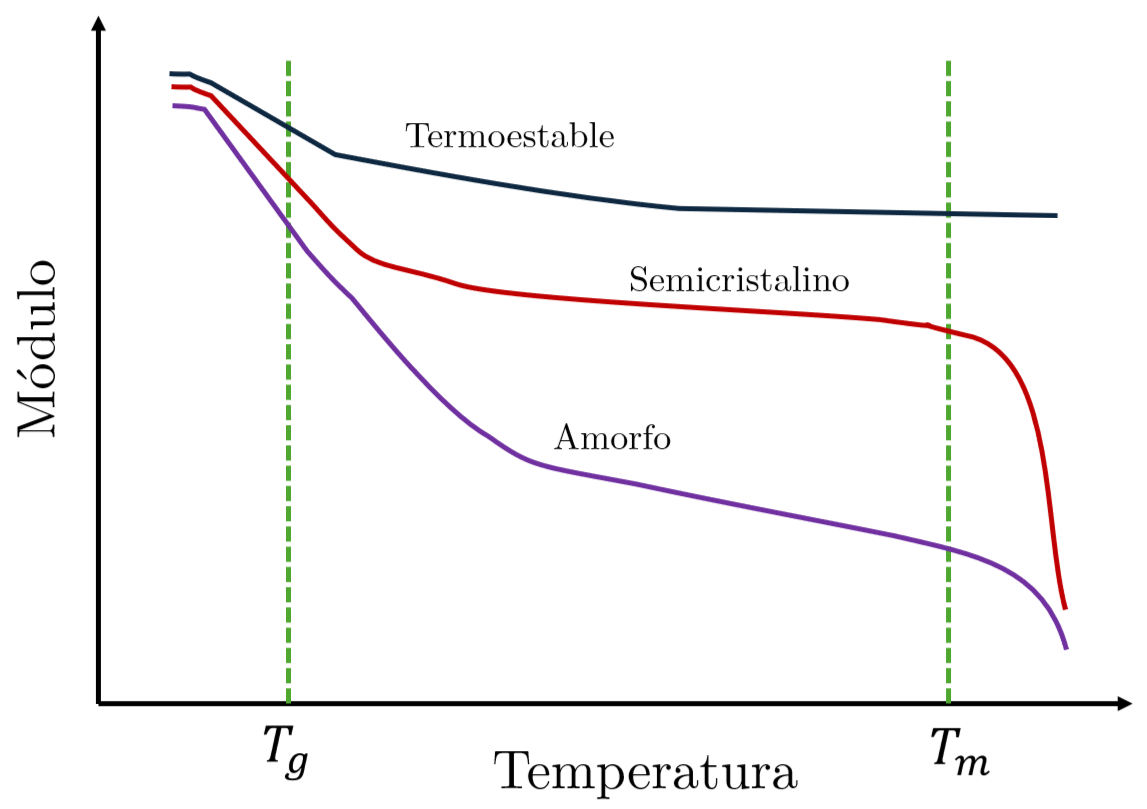
\includegraphics[width=0.7\linewidth]{imgs/tgap.png}
    \caption{Cambio de rigidez con la temperatura en polímeros. La primera línea vertical punteada es la de transición vítrea, la segunda la de fundición.}
    \label{vitr}
\end{figure}

No es posible alcanzar cristalinidad total en polímeros porque sus largas cadenas presentan irregularidades (extremos libres, ramificaciones y defectos) que impiden el empaquetamiento ordenado a lo largo de toda la macromolécula. Además, los entrelazamientos moleculares generan zonas amorfas donde las cadenas no pueden reordenarse en redes cristalinas. Como resultado, siempre coexisten regiones rígidas y ordenadas con áreas desordenadas. En general, los termoestables serán amorfos, pues los enlaces cruzados limita el ordenamiento regular de las cadeas.

En los polímeros semicristalinos, el nivel de cristalinidad (habitualmente un 30–70$\%$) influye en la densidad, la tenacidad y la capacidad de absrober agua (higroscopicidad). Por el contrario, los amorfos suelen presentar una amplia ventana térmica de procesado, lo que facilita operaciones como moldeo por inyección o extrusión.

Cuando un polímero se somete a esfuerzo mecánico, su deformación avanza en varias etapas (Figura \ref{plastens}). Estas dependerán del \textbf{grado de reticulación} (enlaces cruzados) pues limitarán el movimiento de las cadenas, definiendo en parte la ductilidad o fragilidad de un material.

\begin{enumerate}

\item \textbf{Región elástica:} en esta fase inicial la curva esfuerzo–deformación es prácticamente lineal y reversible. Las cadenas poliméricas no se estiran como resortes, sino que giran alrededor de sus enlaces y se reajustan conformacionalmente. Al retirar la carga, la entropía y las rotaciones de enlace devuelven al polímero a su forma original.

\item \textbf{Límite de fluencia:} al superar el esfuerzo lineal máximo, la curva se aplanará o caerá ligeramente. Aquí las cadenas amorfas empiezan a deslizarse unas sobre otras y se inicia la deformación plástica. La muestra ya no recupera completamente su forma al descargar.

\item \textbf{Deformación plástica y necking inicial:} la carga adicional provoca la formación de un cuello en una región localizada. La sección transversal disminuye y las cadenas se reorientan alineándose con la dirección de tracción. El esfuerzo se mantiene alrededor de un valor medio mientras avanza el estrechameiento.

\item \textbf{Endurecimiento por orientación molecular:} tras el necking, la contínua alineación de las cadenas genera un aumento de rigidez. El esfuerzo vuelve a ascender porque las macromoléculas orientadas resisten mejor la carga, exhibiendo un refuerzo mecánico visible en la curva.

\item \textbf{Estrechamiento final y fractura:} la estricción se concentra hasta que la sección remanente ya no soporta más carga. Se produce una caída brusca del esfuerzo y ocurre la rotura. En polímeros dúctiles la superficie de fractura presenta fibrillas o regiones estiradas.

\end{enumerate}

\begin{figure}[h!]
    \centering
    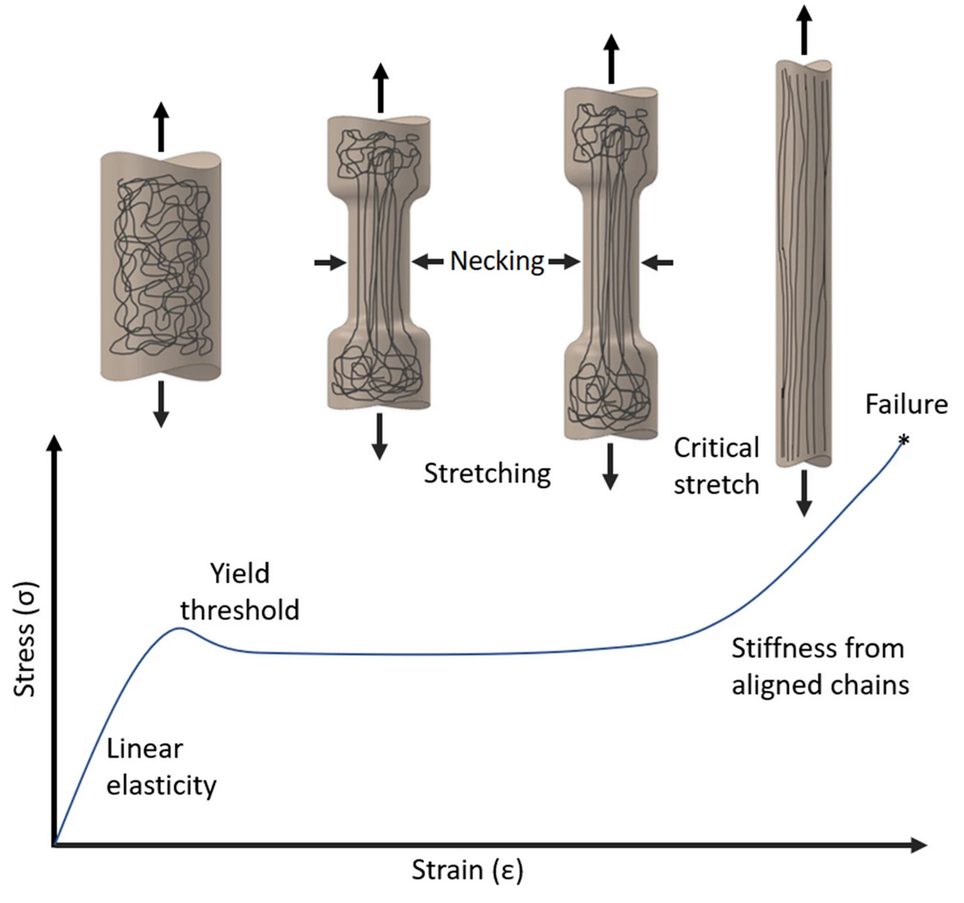
\includegraphics[width=0.7\linewidth]{imgs/estre.png}
    \caption{Curva de esfuerzo-deformación para un polímero dúctil.\cite{tensileplastic}}
    \label{plastens}
\end{figure}

Los polímeros suelen presentar una alta absorción de humedad o \textbf{higroscopicidad} respecto a otros materiales de ingeniería, debido a la presencia de grupos funcionales polares (hidroxilos, ésteres, amidas) en sus cadenas moleculares que establecen enlaces de hidrógeno con el agua.  

Esta captación de humedad impacta negativamente en sus propiedades mecánicas (Figura \ref{humid}) porque las moléculas de agua actúan como \textbf{plastificantes}: aumentan la movilidad de las cadenas poliméricas, reducen el módulo de elasticidad y la resistencia a la tracción, y pueden favorecer la hidrólisis de enlaces, generando microfisuras. Como resultado, se reduce la tenacidad, la estabilidad dimensional y la durabilidad de las piezas.

\begin{figure}[h!]
    \centering
    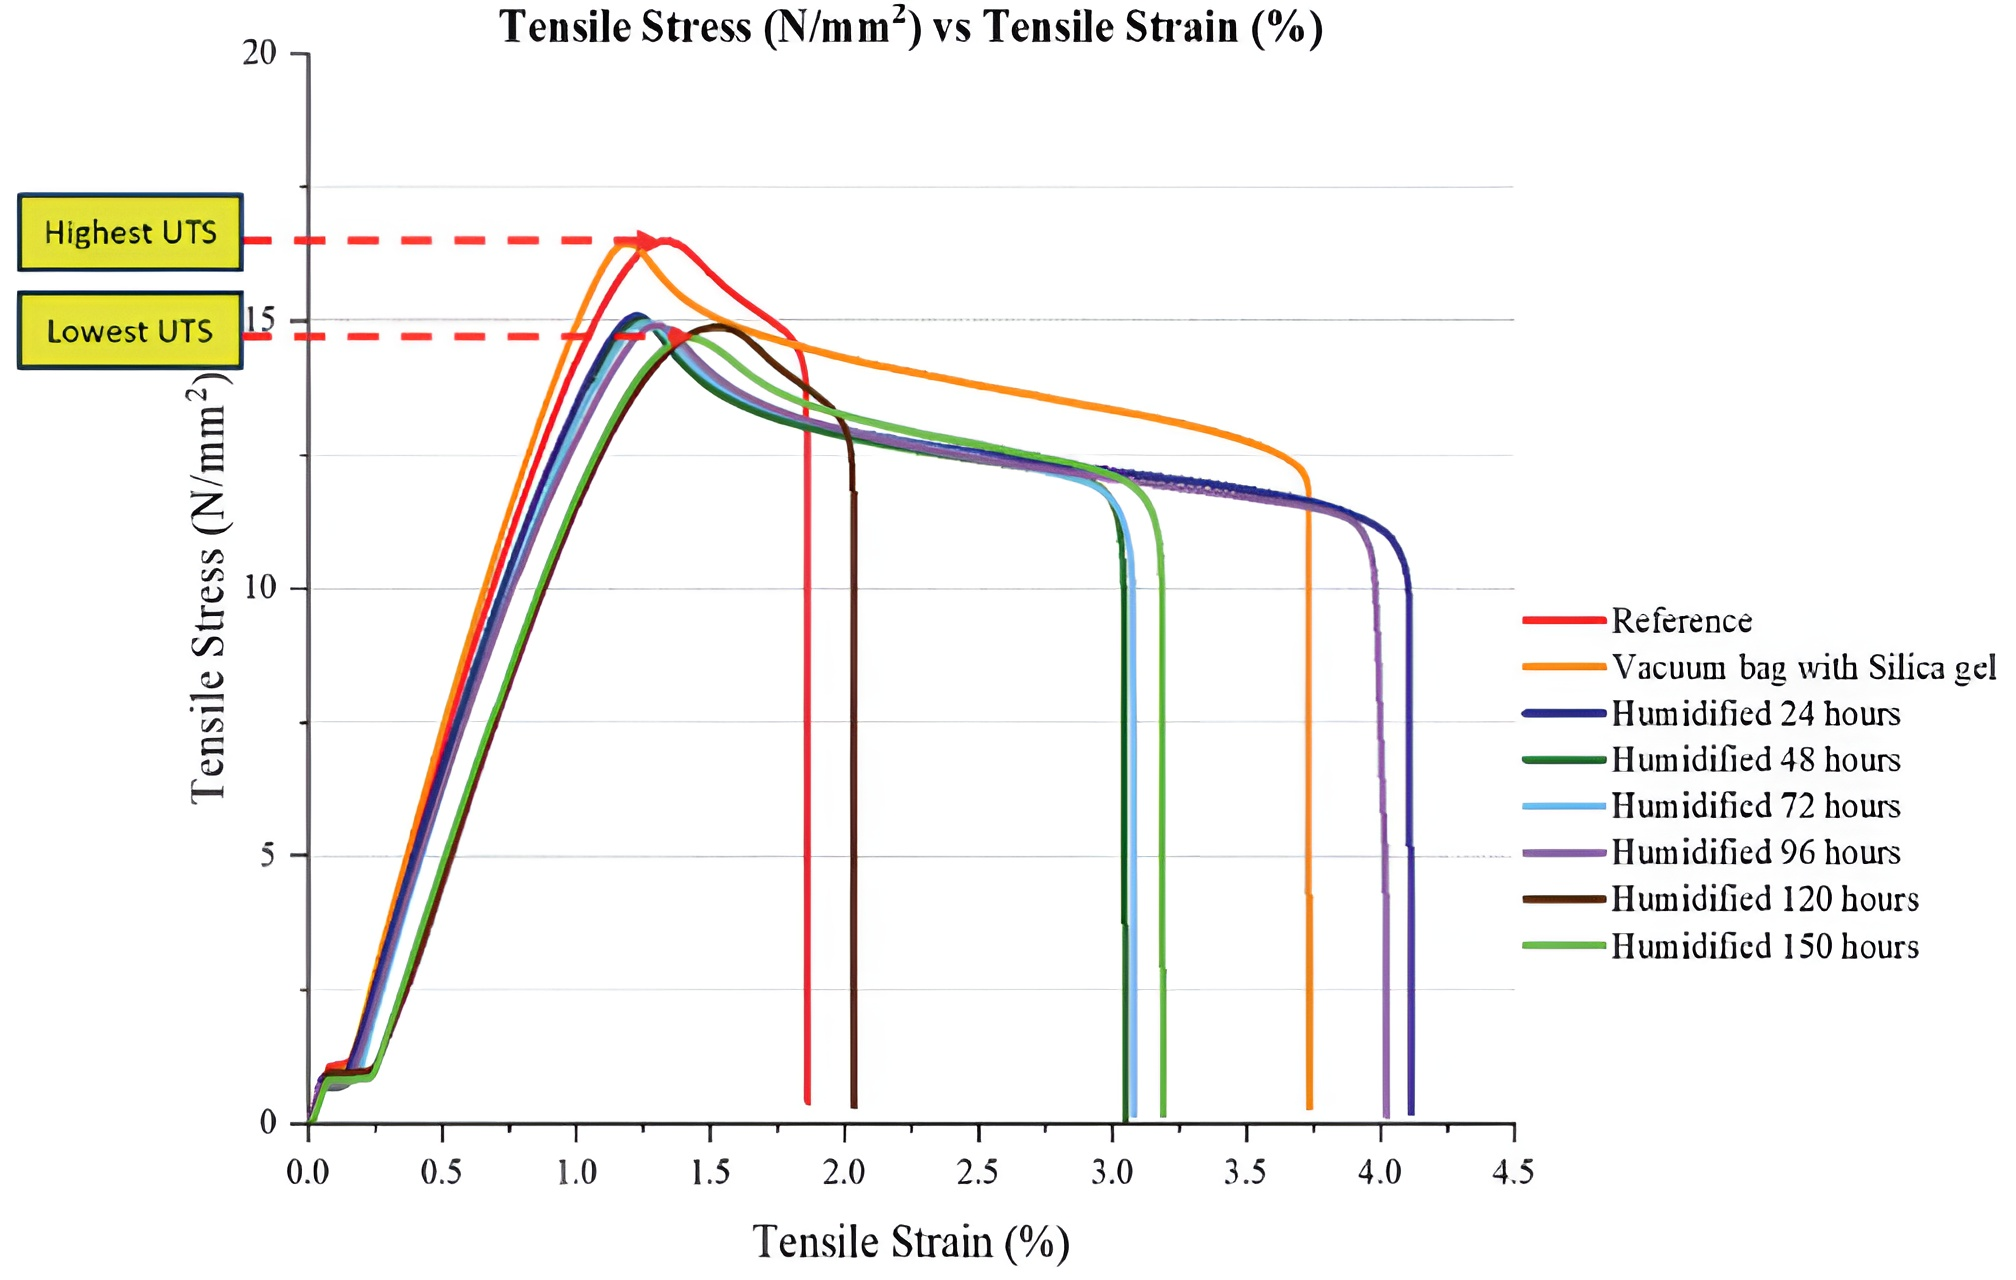
\includegraphics[width=1.0\linewidth]{imgs/humd.png}
    \caption{Gráfico de esfuerzo deformación para un polímero en distintas condiciones de humectación. \cite{jumimi}}
    \label{humid}
\end{figure}

Los polímeros son susceptibles a la \textbf{fotodegradación}, un proceso químico en el cual la radiación ultravioleta (UV) provoca la ruptura de enlaces moleculares. Esto ocurre cuando un electrón absorbe energía UV y pasa a un estado excitado, facilitando la ruptura de enlaces en la cadena polimérica. Los fragmentos resultantes pueden reaccionar con el oxígeno ambiental, contribuyendo a la reducción del peso molecular y a la formación de microplásticos.

En términos de susceptibilidad química, los termoplásticos suelen ser más vulnerables a la fotodegradación debido a la mayor movilidad de sus cadenas moleculares, lo que favorece la formación y propagación de radicales libres que rompen los enlaces. Sin embargo, esta movilidad también permite cierto grado de relajación y reordenamiento molecular, lo que puede mitigar el impacto inmediato sobre sus propiedades mecánicas.

En contraste, los termoestables presentan una estructura reticulada rígida que limita la movilidad molecular y la capacidad de reordenamiento. Esto reduce su susceptibilidad química inicial, pero una vez iniciada la degradación, su fragilidad mecánica aumenta rápidamente debido a la incapacidad de relajar tensiones internas. Así, la resistencia a la propagación de grietas es menor en termoestables que en termoplásticos.

Para reducir el daño potencial asociado a la fotodegradación, es habitual incorporar aditivos estabilizantes durante la fotopolimerización. Estos compuestos actúan como protectores frente a la radiación UV, absorbiendo o disipando la energía dañina y prolongando la vida útil del polímero.
\chapter{Máquinas CNC}

Las máquinas automatizadas de fabricación digital o CNCs son sistemas mecatrónicos programables que ejecutan procesos de manufactura mediante un set de instrucciones definido en un programa. Incluyen tecnologías como la impresión 3D, torneado, fresado, corte láser y robots industriales. Se caracterizan por su precisión, repetibilidad y autonomía operativa, lo que les permite fabricar piezas diversas y complejas de manera sencilla.

\section{Flujo del proceso de fabricación digital}

Las tecnologías de fabricación digital se fundamentan en un proceso computarizado que abarca desde el diseño hasta la producción de la pieza final (Figura \ref{digfab}). Este proceso comienza con la modelación de la componente deseada mediante un software de diseño asistido por computadora (CAD, Computer-Aided Design). Este tipo de herramientas no solo permite crear y visualizar el modelo tridimensional de la pieza, sino también analizar su integración dentro de un sistema ensamblado y evaluar su desempeño mecánico mediante técnicas como el análisis por elementos finitos (FEA, Finite Element Analysis).

\begin{figure}[h!]
    \centering
    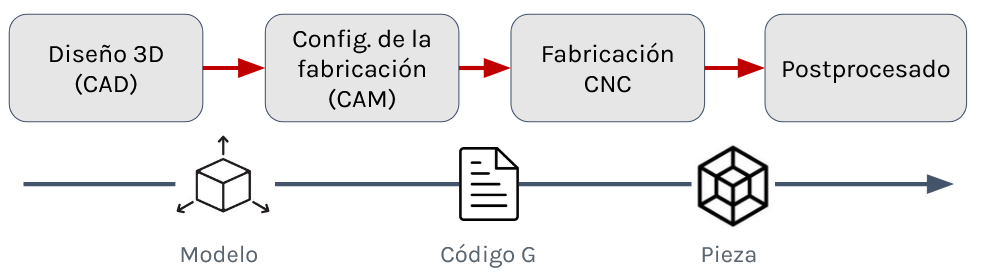
\includegraphics[width=0.9\linewidth]{imgs/digfab.png}
    \caption{Flujo de trabajo para un proceso de fabricación digital.}
    \label{digfab}
\end{figure}

Una vez completado el modelo CAD, este se exporta en un formato de archivo compatible con el software de manufactura asistida por computadora (CAM, Computer-Aided Manufacturing), el cual es específico según el tipo de proceso de fabricación. En el entorno CAM se configuran los parámetros clave del proceso, como velocidades de corte, trayectorias de herramientas y condiciones de operación, con el objetivo de optimizar variables críticas como la calidad del producto final, los costos de producción y el tiempo de fabricación. Además, el software permite simular virtualmente el proceso para verificar su viabilidad, asegurar la compatibilidad con la máquina seleccionada y anticipar posibles errores. Finalmente, el sistema CAM genera un archivo de instrucciones, comúnmente denominado \textbf{código G}, que actúa como entrada para la máquina de fabricación digital, la cual ejecuta el proceso de manera automatizada.

Una vez ejecutados todos los procesos definidos digitalmente, el flujo de trabajo concluye con la etapa de postprocesamiento. Generalmente, esto implica la remoción de la pieza de la máquina y la realización de operaciones complementarias necesarias para alcanzar las condiciones finales del producto. Estas operaciones pueden incluir tareas como el acabado superficial, la limpieza, o la eliminación de estructuras de soporte. En situaciones donde el control de calidad resulta relevante, también se incorpora una fase de metrología para verificar que la pieza cumpla con las especificaciones dimensionales y funcionales establecidas en el diseño.

\section{Sistema}

Cualquier máquina CNC está compuesta de un conjunto de subsistemas primarios (Figura \ref{cncsis}), los cuales generan una \textbf{arquitectura cinemática} (Figura \ref{kinsfig}) de control bidimensional o tridimensional, y subsistemas secundarios, los cuales son de apoyo o específicos del proceso productivo.

\begin{figure}[h!]
    \centering
    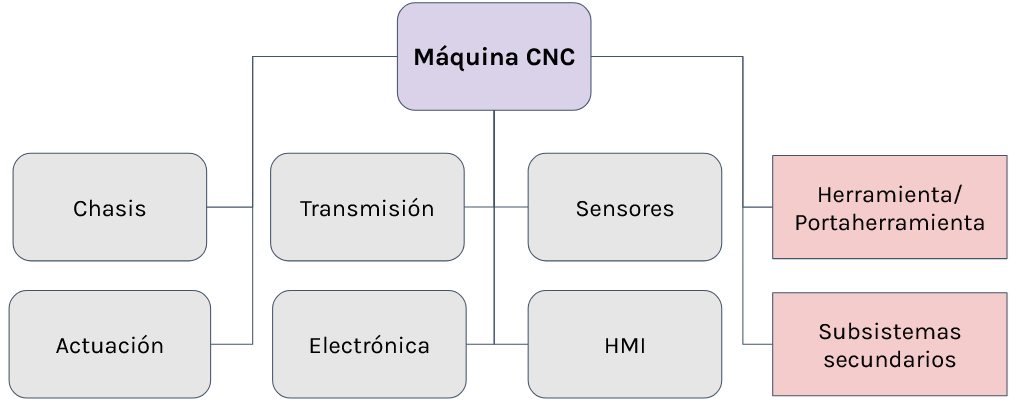
\includegraphics[width=0.9\linewidth]{imgs/cnc.png}
    \caption{Subsistemas en una máquina CNC.}
    \label{cncsis}
\end{figure}

El proceso de fabricación estará determinado por la \textbf{herramienta} o \textbf{portaherramienta} que posea la máquina. Por ejemplo, si se monta un extrusor de plástico la máquina podría funcionar como impresora 3D, y si se cambia por un \textbf{spindle} (portaherramienta rotatorio) la misma máquina podría actuar como fresadora. Si bien, la máquina podría llevar a cabo ambos procesos, la naturaleza de sus subsistemas la hará más idónea para uno de estos.

Entre estos subsistemas primarios se tiene:

\begin{itemize}
    \item \textbf{Interfaz de usuario (HMI):} Permite la comunicación entre el operador y la máquina, para la entrada de comandos, monitoreo de estado y visualización de información relevante. Puede ser una pantalla montada en la máquina, la interfaz de un software o un sistema operativo dedicado.

    \item \textbf{Electrónica:} Incluye al controlador, fuente de poder, y drivers de control de actuadores. Gestiona el procesamiento de señales, comunicación y alimentación. Habitualmente se encuentra como una caja aislada del resto del sistema.

    \item \textbf{Actuadores:} Conjunto de componentes que modifican el estado del sistema, como lo harían motores para el desplazamiento del cabezal en la arquitectura cinemática.

    \item \textbf{Chasis:} Proporciona la estructura mecánica de soporte para el resto de subsistemas. Determina la rigidez, alineamiento y estabilidad durante el funcionamiento de la máquina.

    \item \textbf{Transmisión:} Transfiere el movimiento desde los actuadores hasta los componentes móviles, mediante mecanismos como husillos, correas, engranajes o cremalleras.

    \item \textbf{Sensores/instrumentación:} Capturan información del estado físico de la máquina (posición, temperatura, límites, etc.) para permitir el control del sistema.
\end{itemize}

\begin{figure}[h!]
    \centering
    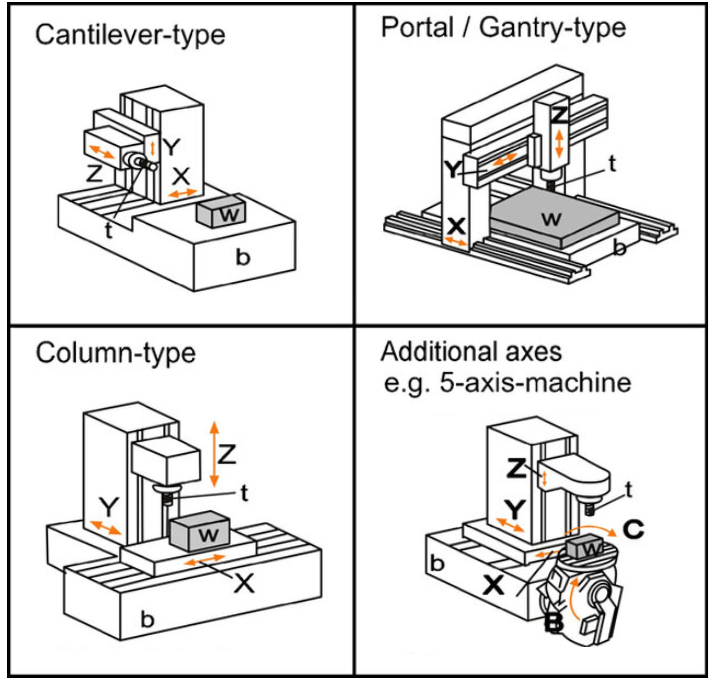
\includegraphics[width=0.67\linewidth]{imgs/kins.png}
    \caption{Ejemplos de arquitecturas cinemáticas.}
    \label{kinsfig}
\end{figure}

\section{Motores stepper}

El control de la posición de un componente o sistema electromecánico suele ser actuado mediante motores eléctricos. La mayoría de los motores eléctricos no otorgan un control directo de la posición de su eje o rotor, sino que es necesario instrumentalizar el sistema con un sensor de tipo \textit{encoder} que mida esta posición y la retroalimente al sistema de control, estableciendo un lazo cerrado (Figura \ref{controlup}). Si bien, esto permitiría un control preciso, el trade-off con la complejidad y costos adquiridos podría no ser conveniente.

\begin{figure}[h!]
    \centering
    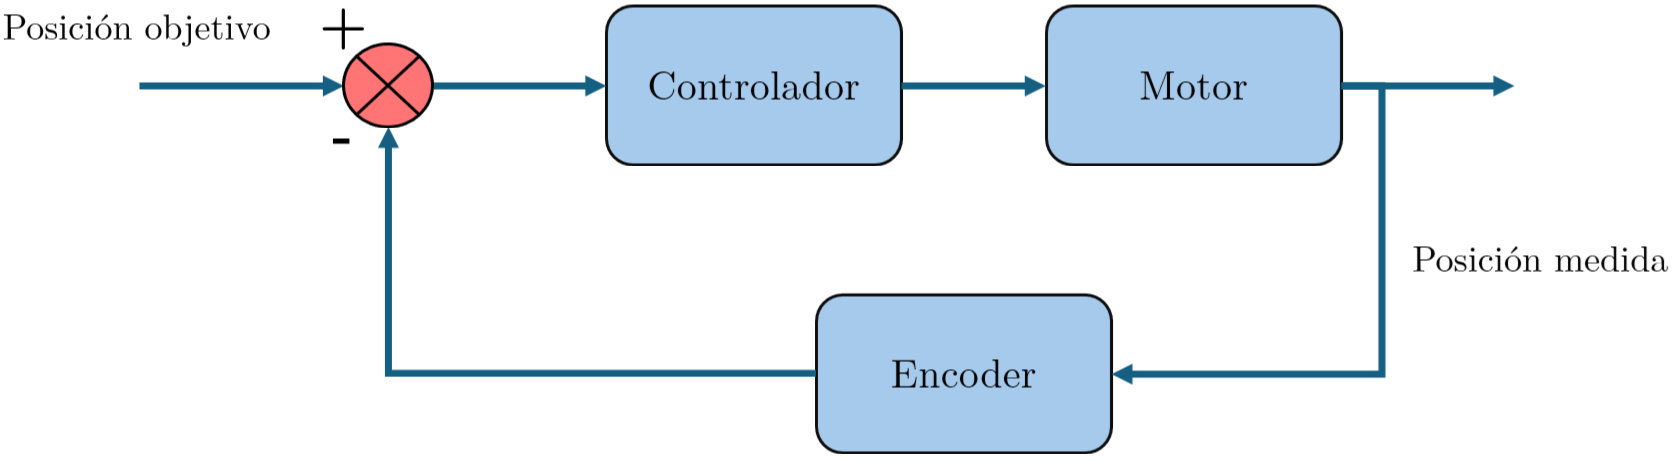
\includegraphics[width=0.9\linewidth]{imgs/controlup.png}
    \caption{Diagrama de control cerrado para controlar la posición de un sistema mediante un motor.}
    \label{controlup}
\end{figure}

Los motores eléctricos de tipo stepper (Figura \ref{stpi}) rotan un arco constante (o un paso, típicamente 1.8$^\circ$) cuando reciben una señal de control. De esta manera, es posible establecer un sistema de control de lazo abierto (sin la parte inferior del loop en la Figura \ref{controlup}) para imponer el perfil cinemático del rotor y la posición final, ofreciendo una opción más sencilla de control. 

\begin{figure}[h!]
    \centering
    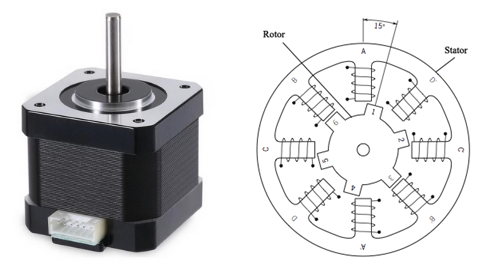
\includegraphics[width=0.7\linewidth]{imgs/stps.png}
    \caption{Motor paso a paso NEMA17 y diagrama de estructura interna.}
    \label{stpi}
\end{figure}

Esto se debe al diseño del motor, en el que el rotor (la parte móvil) está compuesto por un conjunto de imanes permanentes dispuestos de manera intercalada. Estos imanes interactúan con el estator, que consta de bobinas que reciben la señal eléctrica de control. La polarización secuencial de las bobinas genera un campo magnético variable, que provoca el movimiento del rotor, posicionándolo en diferentes puntos de equilibrio. En cada uno de estos puntos, las fuerzas de atracción y repulsión magnéticas se equilibran, permitiendo que el rotor se desplace con precisión o permanezca en una posición fija.

La corriente a través de estas bobinas determinará el torque que puede ejercer el motor contra la carga. En caso de que la carga supere el torque del motor, este no rotará cuando corresponda o se moverá en la dirección opuesta, perdiendo pasos sin que el controlador lo note directamente, induciendo un error en el proceso.

Por lo anterior, versiones más costosas de estos motores incluyen un sistema de sensado, en caso de que la precisión sea crítica o no se trabaje necesariamente en condiciones completamente determinadas.

Los motores paso a paso se clasifican comúnmente según un estándar que define sus dimensiones físicas, particularmente el tamaño de la cara de montaje. Esta clasificación, establecida por la National Electrical Manufacturers Association (NEMA, Figura \ref{nmas}), utiliza números como NEMA 17, NEMA 23, NEMA 34, entre otros, que indican el ancho del marco en décimas de pulgada. Es importante destacar que esta designación solo hace referencia a las dimensiones externas del motor, por lo que dos motores con el mismo número NEMA pueden presentar diferencias significativas en cuanto a torque, corriente nominal, tipo de conexión y otras características eléctricas o mecánicas.

\begin{figure}[h!]
    \centering
    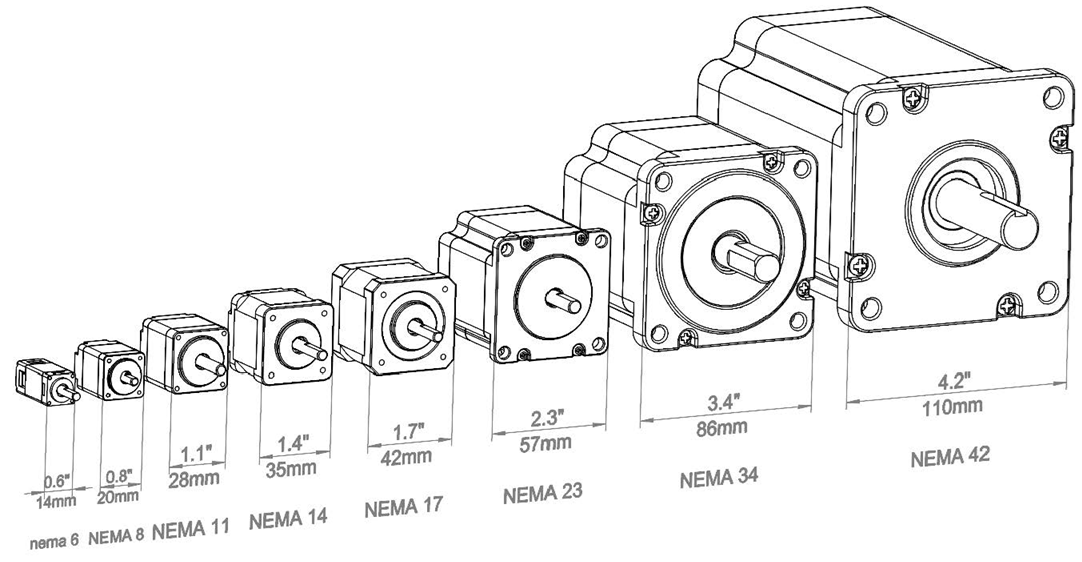
\includegraphics[width=0.9\linewidth]{imgs/nemas.png}
    \caption{Motores paso a paso NEMA.}
    \label{nmas}
\end{figure}

Esta forma de construcción estandarizada brinda flexibilidad al diseño de las máquinas, ya que permite sustituir un motor por otro con las mismas dimensiones de montaje (misma designación NEMA) pero con diferentes especificaciones eléctricas o mecánicas, sin necesidad de realizar modificaciones estructurales, siempre que haya espacio disponible y las condiciones electrónicas lo permitan. Generalmente, los motores NEMA con mayor torque presentan una mayor longitud del cuerpo. Además, existen variantes con diferente ángulo de paso, tipos de eje (plano, estriado, con chavetero), ejes dobles, entre otras configuraciones.

\begin{table}[h]
\centering
\caption{Comparativa estimada de motores paso a paso NEMA. NOTA: Los valores provienen de fabricantes de EEUU, Japón y Alemania, es posible encontrar motores de fabricación China a un tercio del precio pero de prestaciones distintas.}
\label{tab:stepper_nema_comparison}
\begin{tabular}{lccc}
\toprule
\textbf{NEMA} & \textbf{Torque (N·m)} & \textbf{Potencia estimada (W)} & \textbf{Costo aprox. (USD)} \\
\midrule
11 & 0.008 – 0.023 & 1 – 3 & 150 – 170 \\
17 & 0.5 – 0.72 & 10 – 20 & 65 – 95 \\
23 & 0.4 – 3.0 & 20 – 50 & 70 – 130 \\
34 & 4.5 – 12.0 & 50 – 120 & 140 – 220 \\
\bottomrule
\end{tabular}
\end{table}

Mediante la configuración del driver, dispositivo encargado de transformar las señales del controlador en corriente adecuada para las bobinas del motor, es posible ajustar el modo de operación del motor paso a paso, permitiendo dividir cada paso completo en fracciones más pequeñas, como 1/2, 1/4, 1/8, entre otras. Esta técnica, conocida como \textit{microstepping}, permite mejorar la resolución y suavidad del movimiento. No obstante, a medida que se incrementa el nivel de subdivisión, el torque disponible por micro-paso disminuye, debido a que las corrientes aplicadas no alcanzan los valores máximos en cada fase. Por esta razón, si bien el torque total del motor no se reduce, la capacidad de generar fuerza efectiva por paso se ve limitada, especialmente a bajas velocidades.

En una máquina CNC, los motores están físicamente conectados con una transmisión, luego existe una relación entre su desplazamiento rotacional y el de la estructura objetivo, frecuentemente el cabezal o carro. Para un motor que controla la posición en una dirección del cabezal de manera independiente se tiene que:

\begin{equation}
    \Delta x = R\Delta \theta = R n s 
\end{equation}

Donde $\Delta x$ es el desplazamiento en la dirección objetivo, $R$ es la relación de transmisión y $\Delta \theta$ la rotación del eje del motor. Este arco barrido depende de los $n$ pulsos de paso/micropaso que envía el controlador y $s$ el tamaño del paso/micropaso.

\section{Código G}

El código G constituye el lenguaje estándar para la programación de máquinas CNC. Su nombre proviene del hecho de que muchas de sus instrucciones comienzan con la letra G, la cual denota comandos relacionados con operaciones geométricas, como movimientos lineales o circulares. Este conjunto de instrucciones es interpretado por el firmware de la máquina, que lo traduce en movimientos coordinados de los motores a lo largo de los distintos ejes. De esta forma, comandos como el desplazamiento del cabezal a una posición específica en el espacio tridimensional mantienen su significado funcional entre diferentes máquinas CNC, favoreciendo la estandarización del proceso de fabricación digital. No obstante, cada fabricante puede incorporar instrucciones personalizadas o extender el conjunto estándar del código G para incluir funciones específicas de su hardware, lo que requiere adaptar el archivo de instrucciones a las particularidades de cada equipo.

Las instrucciones más comunes son:

\begin{description}[leftmargin=1.5cm, style=nextline]

\item[G0] \textbf{Movimiento rápido}.  
\textit{Sintaxis:} \texttt{G0 X\# Y\# Z\#}  
\textit{Ejemplo:} \texttt{G0 X10 Y5} mueve el cabezal rápidamente a la posición (10, 5). Relacionado con la velocidad máxima o la de movimiento sin fabricar (travel). 

\item[G1] \textbf{Movimiento lineal controlado}.  
\textit{Sintaxis:} \texttt{G1 X\# Y\# Z\# F\#}  
\textit{Ejemplo:} \texttt{G1 X20 Y10 F150} mueve linealmente a (20, 10) con una velocidad de avance de 150 (típicamente, en milímetros por segundo).  

\item[G2] \textbf{Movimiento circular en sentido horario}.  
\textit{Sintaxis:} \texttt{G2 X\# Y\# I\# J\#}  
\textit{Ejemplo:} \texttt{G2 X10 Y10 I5 J0} traza un arco horario hasta (10, 10) con centro relativo en (5, 0).  

\item[G3] \textbf{Movimiento circular en sentido antihorario}.  
\textit{Sintaxis:} \texttt{G3 X\# Y\# I\# J\#}  
\textit{Ejemplo:} \texttt{G3 X10 Y10 I-5 J0} traza un arco antihorario con centro en (-5, 0).  

\item[G20] \textbf{Activar unidades en pulgadas}.  
\textit{Sintaxis:} \texttt{G20}  
\textit{Ejemplo:} \texttt{G20} establece que las dimensiones posteriores estarán en pulgadas.  

\item[G21] \textbf{Activar unidades en milímetros}.  
\textit{Sintaxis:} \texttt{G21}  
\textit{Ejemplo:} \texttt{G21} establece las dimensiones en milímetros (comúnmente usado por defecto).  

\item[G28] \textbf{Ir a posición de referencia (home)}.  
\textit{Sintaxis:} \texttt{G28}  
\textit{Ejemplo:} \texttt{G28} envía el cabezal a la posición de origen de la máquina.  

\item[G90] \textbf{Modo de coordenadas absolutas}.  
\textit{Sintaxis:} \texttt{G90}  
\textit{Ejemplo:} \texttt{G90} hace que las coordenadas se interpreten respecto al origen global.  

\item[G91] \textbf{Modo de coordenadas relativas}.  
\textit{Sintaxis:} \texttt{G91}  
\textit{Ejemplo:} \texttt{G91} hace que las coordenadas se interpreten como desplazamientos relativos desde la posición actual.  

\item[G92] \textbf{Establecer posición actual}.  
\textit{Sintaxis:} \texttt{G92 X\# Y\# Z\#}  
\textit{Ejemplo:} \texttt{G92 X0 Y0 Z0} define la posición actual del cabezal como el nuevo (0, 0, 0).  


\end{description}

En la Figura \ref{g1} se observa un ejemplo sencillo del uso de G1. La herramienta se mueve desde su posición inicial hasta la coordenada (50,100) mediante la instrucción G1 X50 Y100. Al usar G1, en una arreglo cartesiano, por ejemplo, los motores coordinan sus velocidades de acuerdo al parámetro F para detenerse simultáneamente, a pesar de recorrer distancias diferentes. Nótese que el desplazamiento va a depender de si previamente se usó G90 o G91. Si está seleccionado el modo relativo, entonces el desplazamiento será el indicado en G1, pero si el modo es absoluto, el desplazamiento y dirección dependerán de la posición inicial.


\begin{figure}[h!]
    \centering
    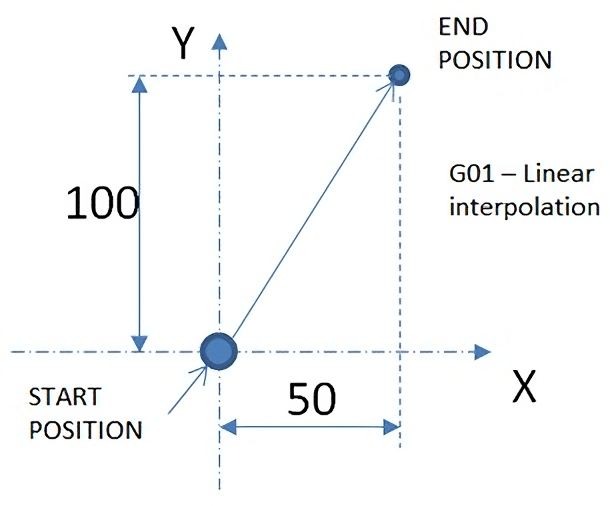
\includegraphics[width=0.5\linewidth]{imgs/g1.png}
    \caption{La instrucción: G1 X50 Y100}
    \label{g1}
\end{figure}


La instrucción G28 \textit{homing} es fundamental para establecer un punto de referencia absoluto desde el cual se medirán los movimientos de la máquina. Este proceso consiste en el desplazamiento automático del cabezal hacia los extremos de los ejes, donde se ubican los sensores de fin de carrera. Estos sensores, de naturaleza digital, detectan la llegada del cabezal y señalan que se ha alcanzado la posición límite predefinida. Una vez completado el procedimiento de homing, el sistema asigna un conjunto de coordenadas a dicha posición, comúnmente el (0,0,0), que pasa a ser el origen del sistema de coordenadas absolutas. A partir de este punto, es posible establecer orígenes relativos adicionales (G92), lo que resulta útil para optimizar ciertos procesos de fabricación, en particular aquellos que requieren operaciones repetitivas o el uso de dispositivos de montaje. Es posible hacer homing de los ejes de manera independiente, indicándolo en la instrucción (G28 X, por ejemplo).

El conjunto restante de códigos disponibles dependerá del tipo de proceso de fabricación implementado en cada máquina, así como de sus capacidades específicas y del grado de personalización definido por el fabricante. Estos códigos adicionales permiten ejecutar instrucciones complementarias, tales como el cambio automático de herramientas, el calentamiento de determinados componentes, la activación de sistemas de refrigeración, entre otras funciones necesarias para la operación del equipo.

\section{Capacidades y performance}

Uno de los parámetros más relevantes en la fabricación de una pieza es la velocidad de operación, la cual está condicionada por diferentes factores, como por ejemplo, las capacidades de los motores que componen la cadena cinemática del sistema. Si bien el objetivo suele ser minimizar el tiempo de producción aprovechando al máximo el rendimiento de los motores, un aumento en la velocidad puede generar efectos adversos. En particular, fenómenos de naturaleza mecánica, como las vibraciones o las resonancias estructurales, pueden comprometer la precisión y la calidad superficial de la pieza final.

Estos fenómenos están directamente relacionados con la construcción de la máquina y las características específicas del proceso. La rigidez global del chasis, la robustez y precisión del sistema de transmisión, la capacidad de amortiguación de la estructura, la alineación correcta entre ejes durante el ensamble, y las inercias asociadas a los componentes móviles determinan en gran medida la \textbf{respuesta dinámica del sistema}. Una estructura con baja rigidez puede experimentar deformaciones ante cargas dinámicas, mientras que transmisiones con \textbf{juego mecánico} o flexibilidad excesiva introducen errores en la trayectoria programada. Asimismo, inercias elevadas dificultan las aceleraciones controladas, y una amortiguación insuficiente puede prolongar oscilaciones no deseadas tras cambios bruscos de velocidad o dirección.


\begin{figure}[h!]
    \centering
    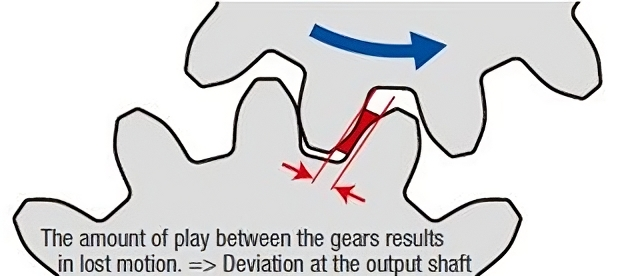
\includegraphics[width=0.7\linewidth]{imgs/gears.png}
    \caption{Juego mecánico entre dos engranajes.}
    \label{gears}
\end{figure}

El juego mecánico (backlash, en inglés) se refiere al movimiento relativo no deseado entre dos componentes mecánicos cuando se invierte la dirección del movimiento en un sistema de transmisión. Este fenómeno ocurre, por ejemplo, en engranajes, husillos, tuercas o acoplamientos, y se manifiesta como un pequeño desplazamiento libre antes de que el movimiento se transmita efectivamente. No es viable eliminar completamente el juego mecánico, es consecuencia de \textbf{tolerancias} de fabricación, desgaste o diseño intencional, y puede afectar negativamente la precisión y repetibilidad en sistemas de control numérico y máquinas de fabricación digital. Una característica positiva del juego mecánico es facilitar o hacer posible el ensamble de un sistema.

La tolerancia en un proceso de fabricación se define como la variación dimensional permitida respecto a las especificaciones nominales de una pieza, dentro de la cual el componente aún se considera funcional y conforme al diseño. Representa el rango aceptable de desviaciones en dimensiones lineales, angulares, formas o posiciones, y se establece en función de los requerimientos de ensamblaje, desempeño mecánico y costos de producción. Las tolerancias son un elemento clave en el control de calidad, ya que determinan los límites dentro de los cuales un proceso puede producir piezas sin necesidad de retrabajo o descarte. Por ejemplo, una tolerancia común en impresoras 3D de escritorio tipo FDM es de $\pm 0.5 \,\mathrm{mm}$, lo cual debe tomarse en cuenta al momento del diseño, especialmente para asegurar encajes.

Otra característica deseada en un proceso de fabricación es la precisión, nuevamente, determinada por la construcción de la máquina y el tipo de operaciones desarrolladas. En el contexto de manufactura, es importante distinguir entre \textbf{precisión} y \textbf{exactitud} (accuracy) (Figura \ref{press1}). La precisión se refiere a la consistencia de los resultados: una máquina es precisa si produce piezas con dimensiones muy similares entre sí, aunque todas estén ligeramente desviadas del valor nominal. En cambio, la exactitud indica qué tan cerca está el resultado del valor deseado o teórico. Por ejemplo, si una impresora 3D fabrica diez piezas de 20 mm y todas miden 19,7 mm, decimos que es precisa (porque es repetitiva), pero no exacta (porque hay un error sistemático).

\begin{figure}[h!]
    \centering
    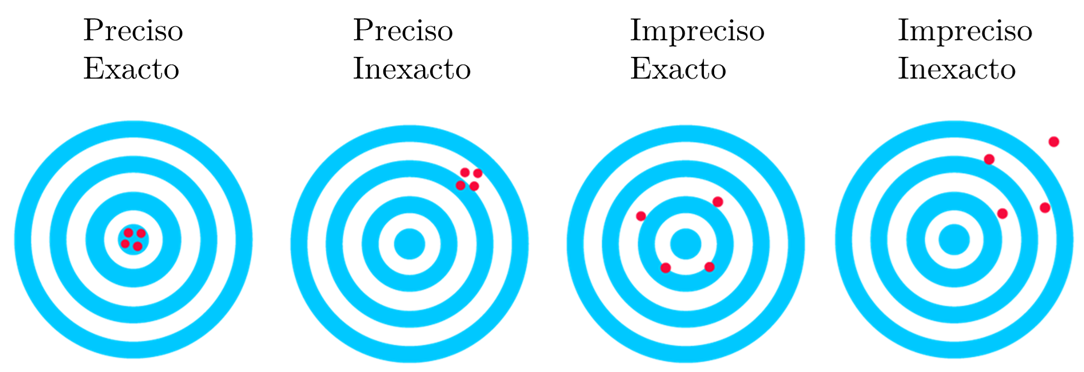
\includegraphics[width=0.9\linewidth]{imgs/press.png}
    \caption{Precisión y exactitud. La precisión se mide como la dispersión entre puntos, y la exactitud respecto al objetivo.}
    \label{press1}
\end{figure}

En una arquitectura cinemática basada en motores paso a paso, el error de exactitud está condicionado por la naturaleza discreta del paso angular. Cada pulso desplaza el eje un ángulo fijo, introduciendo un sesgo sistemático de hasta $\pm \tfrac{1}{2}$ paso o micropaso frente al valor de consigna. De este modo, ciertas posiciones teóricas resultan inalcanzables para el sistema; no obstante, la importancia de este sesgo depende de la tolerancia admitida en el proceso.

Al igual que los motores paso a paso, la instrumentación digital, a través de encoders incrementales o absolutos y convertidores analógico-digitales (ADC), introduce un error de cuantización fijo, determinado por su resolución espacial y digital: la señal analógica se discretiza en incrementos, generando un sesgo máximo de $\pm ½$ LSB (Least Significant Bit). Al mismo tiempo, el sistema de control ejecuta su loop de realimentación con una frecuencia de muestreo y actualización finitas, lo que provoca retardos equivalentes a un periodo de muestreo y variaciones de temporización (jitter) en la emisión de pulsos de actuación. Estos efectos combinados, cuantización de la instrumentación y discretización temporal del controlador, se traducen en errores sistemáticos y aleatorios de seguimiento de trayectoria, limitando la exactitud dinámica y la repetibilidad del proceso.

Finalmente,en la fase operativa de fabricación surgen múltiples fuentes de error inherentes al material y a la herramienta. Por ejemplo, el filamento de impresión 3D puede presentar variaciones de diámetro a lo largo de la bobina, además de absorber humedad o contener impurezas, lo que provoca fluctuaciones en el caudal de extrusión. Por otro lado, las herramientas de corte experimentan dilatación térmica y deflexión mecánica bajo carga y temperatura elevadas, generando desplazamientos sistemáticos en el perfil de la pieza y afectando la rugosidad de la superficie.

Así, en la fabricación por CNC, el componente real rara vez reproduce con exactitud el modelo diseñado debido a la confluencia de múltiples fuentes de imprecisión inherentes al proceso. Estas desviaciones, que emergen de la interacción entre la respuesta dinámica de la máquina, la resolución del sistema de control y la instrumentación digital y las condiciones operativas del mecanizado, deben anticiparse desde la fase de diseño geométrico y de tolerancias hasta la selección y ajuste de la máquina. De este modo, se asegura que las tolerancias dimensionales y la calidad superficial esperadas sean coherentes con el comportamiento efectivo del sistema CNC.

\section{Prototipado rápido}

En las primeras fases del desarrollo de un producto, el prototipado transforma ideas y bocetos en modelos físicos de baja fidelidad que evolucionan progresivamente hacia versiones cada vez más representativas. Este proceso culmina en un nivel de confianza suficiente para planificar la producción con seguridad. El prototipado rápido (Figura \ref{propro}) destaca como una metodología ágil al emplear máquinas de fabricación digital capaces de materializar directamente diseños CAD.

\begin{figure}[h!]
    \centering
    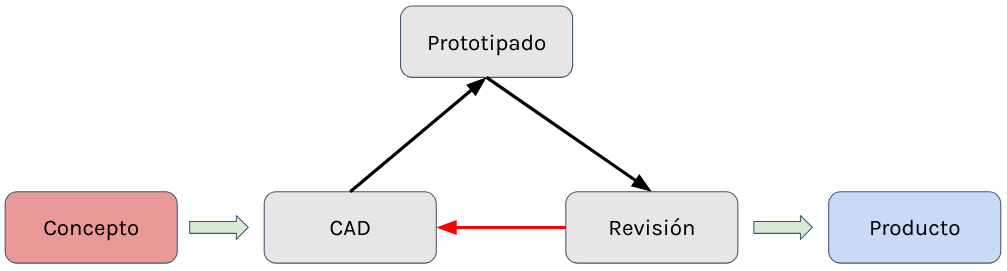
\includegraphics[width=1.0\linewidth]{imgs/prototip.png}
    \caption{Flujo de la metodología de prototipado rápido.}
    \label{propro}
\end{figure}

La visualización 3D en el CAD complementada con los módulos de análisis y simulación mecánica refuerza la confianza en la viabilidad del diseño y evita asumir prematuramente los costes de fabricación. Aunque el entorno 3D permite anteponerse incluso a obstáculos de ensamble, no puede entregar toda la información que se obtendría manipulando una maqueta o modelo a escala del producto.

Según la tecnología de fabricación digital empleada, ya sea una impresora 3D FDM de escritorio o un centro de mecanizado industrial, se pueden obtener diferentes tipos de prototipos adaptados a cada objetivo: maquetas para validar ensamblajes e interacción, piezas de alta fidelidad con acabado superficial equiparable al de un molde de inyección, o réplicas en el material definitivo para ensayos de servicio, o incluso, de manufactura.

La selección del proceso de manufactura definitiva es un paso esencial para cerrar el diseño de un producto. Aunque la fabricación digital acelera la validación de conceptos, rara vez resulta competitiva en costes al escalar a producción en serie. Sin embargo, la flexibilidad de estas tecnologías permite crear prototipos cuyas geometrías incorporan de antemano las restricciones y oportunidades de los métodos productivos finales, poniendo en práctica un enfoque de \textbf{diseño orientado a la manufactura}.
\chapter{Tecnologías de manufactura aditiva}

\section{Introducción}

Llamaremos procesos de manufactura aditiva a todas las técnicas en las que el material se \textbf
{deposita de forma controlada} y capa a capa sobre un volumen de trabajo para construir directamente geometrías tridimensionales. 

La construcción secuencial elimina restricciones de trayectoria (colisiones, cambios de herramienta) propias de máquinas-herramienta convencionales y fusiona varias etapas de fabricación en un único paso. Además, como las fuerzas involucradas son muy bajas, los equipos pueden diseñarse con menor tamaño y potencia, reduciendo costes energéticos, de infraestructura y seguridad.

Las tecnologías de manufactura aditiva suelen poseer las siguientes características en común:

\begin{description}

\item[Versatilidad geométrica]  
    No tienen restricciones de forma o un enfoque especializado, como sí sucede con un torno (simetría circular) o una fresa (geometrías rectas).

  \item[Capacidad para producir geometrías complejas] 
    Permite generar estructuras reticuladas, cavidades internas y perfiles orgánicos inviables o excesivamente costosos mediante técnicas sustractivas, ampliando el campo de optimización topológica.

  \item[Producción bajo demanda] 
    Al eliminar la necesidad de utillajes y moldes específicos, habilita la fabricación inmediata de piezas según requerimientos puntuales, reduciendo inventarios y tiempos de espera ante modificaciones de diseño.

  \item[Requisitos de formación técnica accesibles] 
    Las plataformas aditivas suelen incluir interfaces gráficas y flujos de trabajo asistidos que facilitan la preparación de archivos de impresión sin necesidad de capacitación avanzada en programación de máquinas.

  \item[Repetibilidad y copias idénticas] 
    El control preciso de parámetros como temperatura, caudal de material y trayectoria de deposición asegura la fidelidad entre el modelo digital y la pieza final, garantizando una producción homogénea.

  \item[Portabilidad y tamaño compacto] 
    Existen sistemas aditivos de dimensiones reducidas que pueden instalarse en talleres, laboratorios de investigación o entornos de campo, lo que facilita el prototipado rápido y la movilidad.

  \item[Combinación de materiales] 
    Algunas tecnologías permiten depositar de manera simultánea o secuencial diferentes tipos de polímeros, resinas o metales, generando gradientes de propiedades mecánicas, térmicas o eléctricas.

  \item[Reducción de material de desecho] 
    Al construir componentes únicamente con el volumen necesario, disminuye significativamente los recortes y rebabas propios de procesos sustractivos, optimizando la utilización de materia prima.
    
\end{description}

Estas características convierten a la manufactura aditiva en una alternativa sumamente atractiva para modelos productivos flexibles: las modificaciones de diseño se incorporan sin alteraciones en la cadena de suministro, los inventarios pueden reducirse o eliminarse por completo y el aprovechamiento de la materia prima se maximiza. Sin embargo, su principal hándicap reside en la \textbf{velocidad de fabricación}. Al operar mediante deposición secuencial capa por capa, el tiempo de proceso crece de forma casi lineal con el tamaño y la complejidad de la pieza. Además, tratar de acelerar la tasa de deposición suele comprometer la resolución y la calidad del acabado superficial, lo que atenúa buena parte de la ventaja diferencial de esta tecnología.

La evolución del volumen de producción de un componente o producto define el punto de equilibrio en el que los sistemas flexibles de manufactura (por ejemplo, centros CNC) dejan de ser competitivos frente a maquinaria altamente especializada. En lotes pequeños o medianos, la ausencia de conjuntos de herramientas y la capacidad de reconfiguración rápida de CNC y manufactura aditiva ofrecen tiempos de respuesta reducidos y bajos costos iniciales. Sin embargo, a medida que el tamaño del lote supera un umbral crítico (\(q^*\)), la inversión en moldes, troqueles o líneas automatizadas amortiza su alto coste inicial mediante ciclos unitarios extremadamente rápidos y costos marginales decrecientes.  

En consecuencia, la manufactura aditiva despliega su mayor ventaja competitiva en nichos de mercado caracterizados por:

\begin{itemize}
  \item \textbf{Producción on-demand} de piezas personalizadas (por ejempllo, prótesis y órtesis a medida), donde cada muestra requiere geometrías únicas.  
  \item \textbf{Componentes aeroespaciales} con topologías optimizadas para relación resistencia-peso y cavidades internas complejas.  
  \item \textbf{Herramientas de serie corta y prototipos funcionales} en proyectos de I+D, donde la flexibilidad de diseño y la velocidad de iteración priman sobre el coste unitario.  
  \item \textbf{Piezas de edición limitada} en sectores como automoción de alta gama o diseño industrial, donde el valor añadido justifica tiempos de fabricación superiores.
\end{itemize}  

Aunque la manufactura aditiva presenta ciertas restricciones para su producción industrial a gran escala, especialmente en términos de tiempos de ciclo y costo unitario, resulta una herramienta inigualable durante la fase de prototipado, razón principal para el nacimiento de estas tecnologías.

\subsection{Tipos de tecnologías}

Bajo la definición anterior, las familias generales de tecnologías de manufactura aditiva son:

\begin{itemize}
  \item \textbf{Vat photopolymerization:}  
    fotopolimerización selectiva de una resina líquida en un tanque mediante un haz de luz (láser o proyector). Cada capa se cura en la zona expuesta, obteniéndose piezas con alta resolución y excelente acabado superficial. Materiales típicos: resinas acrílicas, epóxicas o híbridas.

  \item \textbf{Material extrusion:}  
    extrusión de material termoplástico, cerámico, metálico (filamento o pasta) a través de una boquilla calentada. El cordón depositado se funde y solidifica capa a capa. Materiales típicos: PLA, ABS, Nylon, pastas cerámicas o compuestos cargados.

  \item \textbf{Material jetting:}  
    depositado por inyección de gotas de material (resinas, cerámicas, ceras o metales) a través de cabezales piezoeléctricos, seguido de fotopolimerización o fusión local. Permite impresión multi-material y gradientes de propiedades en una misma pieza.

  \item \textbf{Binder jetting:}  
    chorro de un aglomerante líquido sobre un lecho de polvo (polímero, metal o cerámico) para aglomerar selectivamente las zonas deseadas. Tras la impresión, la pieza en verde se cura o sinteriza para densificarla. Materiales típicos: acero, aluminio, arena de sílice, polvos cerámicos.

  \item \textbf{Powder bed fusion:}  
    fusión o sinterizado selectivo de un lecho de polvo mediante un láser o haz de electrones. El polvo sinterizado actúa de andamiaje, eliminando la necesidad de soportes. Materiales típicos: poliamidas, polietileno, aleaciones de aluminio, acero, titanio.

  \item \textbf{Direct energy deposition:}  
    alimentación simultánea de polvo o alambre con un haz de energía (láser, electrones, plasma) que funde el material en el punto de deposición. Ideal para reparaciones y recubrimientos de componentes metálicos. Materiales típicos: aceros inoxidables, aleaciones de titanio, superaleaciones.

  \item \textbf{Sheet lamination:}  
    unión de láminas de material (papel, polímero, metal o compuestos) mediante adhesivos, soldadura láser o ultrasonidos, y corte secuencial de cada capa para formar la geometría final. Materiales típicos: acero laminado, aluminio, papel tratado, polímeros.
\end{itemize}

Cada una de estas tecnologías de manufactura aditiva presenta atributos particulares que las hacen idóneas para aplicaciones específicas. La selección de la tecnología más adecuada debe fundamentarse en la combinación de parámetros como el tipo de material, la resolución requerida, el coste unitario y el volumen de producción.  

Gran parte de estas máquinas ha experimentado una evolución estructural análoga a la de los computadores: de voluminosos sistemas industriales, costosos y de manejo complejo, a una amplia oferta de modelos de escritorio, asequibles y de operación intuitiva. Esta transformación se ha materializado principalmente en las dos tecnologías aditivas más populares, extrusión y fotopolimerización en vat, impulsadas por el movimiento maker, el desarrollo de plataformas open-source y la diversificación de materiales compatibles.

\subsection{Slicer}

En el flujo de trabajo de fabricación aditiva, el software CAM incorpora un módulo slicer que segmenta el modelo 3D en $n$ planos horizontales (paralelos al eje $x-y$). Cada uno de estos cortes tiene un espesor igual al parámetro operativo de \textbf{altura de capa} y será la unidad básica que se apile durante la impresión para reconstruir la geometría del diseño.

La altura de capa es un parámetro crítico: define la resolución y la fidelidad geométrica de la pieza, y condiciona el tiempo total de fabricación. Una capa más delgada mejora el detalle superficial y la precisión dimensional, pero exige más pasadas de extrusión y prolonga el tiempo de impresión. En cambio, capas más gruesas aceleran el proceso a costa de perder definición en detalles finos.

Sobre cada sección transversal generada, el slicer traza la trayectoria de la herramienta (toolpath) y genera el código G correspondiente en función del resto de parámetros operativos a configurar en el CAM.

El archivo que se importa al slicer rara vez conserva el formato nativo del CAD (por ejemplo, STEP o IGES); en su lugar se convierte la superficie del modelo en una malla poligonal que la aproxima, normalmente mediante un archivo con extensión .stl. En este formato, la geometría 3D se tesela en triángulos: las curvas y detalles se aproximan con facetas planas, pero se pierde por completo la información volumétrica interna (materiales, estructuras huecas o sólidos). El acrónimo STL se interpreta habitualmente como Stereolithography, Standard Tessellation Language o Standard Triangle Language. 

El grado de refinamiento de esa malla condiciona la fidelidad entre el diseño original y lo que realmente procesa el slicer: una malla demasiado gruesa produce polígonos (facetas) visibles, mientras que una demasiado densa no mejora la calidad de impresión, pues la impresora tiene una resolución limitada. Es clave elegir un nivel de detalle óptimo que equilibre precisión y eficiencia computacional.

Este archivo sólo describe la envolvente externa de la pieza; no incluye información sobre su volumen o espesores interiores. Estas características serán definidas mediante los parámetros del CAM a utilizar.

\section{Impresión 3D por extrusión}

\subsection{Modelado por deposición fundida}

Esta tecnología de manufactura se basa en la deposición controlada de material a través de una boquilla dispensadora. Su aplicación más común es la impresión con filamento termoplástico: un motor impulsa el hilo hacia un módulo de calentamiento que aplica un perfil térmico preciso. De este modo, el polímero permanece rígido durante el avance y se ablanda al atravesar la zona caliente, alcanzando la viscosidad óptima para su extrusión controlada.

Una vez depositado el material, este se solidifica casi de inmediato en el lugar donde fue extruido (idealmente), enfriándose y recuperando rigidez. Esto se repite capa a capa hasta construir la geometría deseada.

La impresora emplea una arquitectura cinemática tridimensional, diseñada para mover el cabezal sin necesidad de fuerzas elevadas, más allá de las requeridas para vencer su propia inercia. La masa móvil depende de la posición del motor de extrusión, que puede situarse dentro del cabezal (\textbf{extrusión directa}) o en un soporte externo (\textbf{sistema Bowden}).

El sistema Bowden reduce significativamente la masa del cabezal, disminuye la inercia y permite mayores aceleraciones con menos vibraciones. En cambio, el extrusor directo, al llevar el motor integrado en el cabezal, minimiza el roce y la deformación del filamento, mejorando la calidad de la extrusión, especialmente con materiales flexibles.

El cabezal cuenta con diversas componentes, encargadas de dirigir el filamento y otorgar el gradiente térmico:

\begin{itemize}
  \item \textbf{Calefactor y termocupla}: Este par permite aplicar y mantener con precisión el perfil térmico necesario para fundir el filamento.

  \item \textbf{Disipador}: bloque de aluminio con aletas diseñado para extraer el calor en el cabezal y evitar el paso de este hacia la zona fría. Garantiza que el filamento se mantenga rígido hasta llegar al bloque calefactor, previniendo atascos.

  \item \textbf{Ventilador}: montado sobre el disipador, impulsa aire en las aletas para optimizar la extracción de calor. 

  \item \textbf{Ventilador de capas}: enfoca un flujo de aire directo sobre la pieza impresa, acelerando la solidificación del plástico extruido. 

  \item \textbf{Boquilla}: punta de latón, acero o acero endurecido con un orificio calibrado (generalmente de 0.4 mm). Controla el flujo de material fundido y define la resolución, el ancho de línea y el volumen de extrusión de cada capa.
\end{itemize}

Esta técnica de impresión es actualmente la más popular, pues la simplicidad de la máquina y el costo de los materiales permite que existan modelos de escritorio de alrededor de unos cien dólares.

En la impresión FDM, el plástico se deposita sobre una \textbf{plataforma o cama}, que puede ser fija o móvil según la arquitectura cinemática de la impresora. La adhesión de la primera capa es crítica, pues de ella depende la estabilidad de todo el conjunto; el fallo más habitual es el despegue de la pieza durante la impresión. Para optimizar el contacto, la boquilla debe quedar perfectamente perpendicular a la superficie de la cama. Esta nivelación se logra mediante calibración manual, sistemas de nivelación automática o ajustes adaptativos por sensores, según el modelo de impresora. 

La adhesión del plástico ocurre al fluir el plástico caliente entre los micro relieves de la cama, anclándose mecánicamente. Además, esta adhesión podría ser favorecida cuando existe afinidad química o polar entre el polímero y el material de la base. La plataforma de impresión puede presentar distintas rugosidades: una superficie texturizada favorece la adherencia del filamento, pero está sujeta a desgaste, mientras que el vidrio liso proporciona un acabado más pulido y durabilidad, pero es más difícil la adhesión.

El despegue de la pieza suele originarse por \textbf{warping}, un fenómeno en el que los gradientes térmicos durante el enfriamiento generan tensiones internas que deforman y curvan los bordes, separándolos de la cama. Para contrarrestar este efecto, la plataforma se calienta hasta una temperatura cercana al punto de transición vítrea del polímero. Así, la pieza se enfría de forma más gradual y permanece más flexible, reduciendo las tensiones por contracción térmica. Algunos modelos de impresoras presentan un \textbf{ambiente cerrado}, el cual puede incluso contar con control de temperatura, controlando mejor los gradientes térmicos generados durante el proceso.

Al elegir un material para impresión FDM, resulta fundamental entonces que su \textbf{coeficiente de dilatación térmica} sea bajo. Esta característica minimiza el warping y refuerza la precisión dimensional al reducir la variación de volumen durante el enfriamiento. Por ello, el coeficiente de dilatación es un parámetro clave para la facilidad de impresión o \textbf{imprimibilidad} de un polímero. Existen otras propiedades mecánicas que influyen en el proceso, pero suelen requerir compromisos, cada una tiene una ventana óptima de funcionamiento en lugar de un valor extremo universal.

\begin{table}[h]
  \centering
  \footnotesize
  \begin{tabular}{|p{3cm}|p{5cm}|p{5cm}|}
    \hline
    \textbf{Propiedad} & \textbf{Muy baja} & \textbf{Muy alta} \\
    \hline
    Coeficiente de dilatación térmica (\(\alpha\)) 
      & Contracción casi nula y mínima deformación térmica 
      & Elevadas tensiones internas, warping pronunciado y despegue de bordes \\
    \hline
    Difusividad térmica 
      & Gradientes térmicos marcados, warping localizado y mala unión intercapas 
      & Enfriamiento demasiado rápido, fusión insuficiente entre capas \\
    \hline
    Viscosidad fundida 
      & Filamento excesivamente fluido: colapso de voladizos y goteo constante 
      & Extrusión irregular, obstrucciones y falta de flujo uniforme \\
    \hline
    Adhesión intercapas 
      & Delaminación, baja resistencia mecánica y capas sueltas 
      & Sobrellenado, pérdida de detalle en bordes y posibles deformaciones \\
    \hline
    Elongación a rotura (\(\%\)) 
      & Piezas frágiles, fisuras y roturas en puentes y voladizos 
      & Deformaciones postimpresión, tendencia a serpentear o estirarse bajo peso \\
    \hline
    Módulo de elasticidad (\(E\)) 
      & Capas se arquean bajo su propio peso y geometría inestable 
      & Estructuras rígidas y quebradizas, propagación rápida de grietas \\
    \hline
    Temperatura de transición vítrea (\(T_g\)) 
      & Material blando en impresión: deformaciones y colapso de detalles 
      & Difícil soldado de capas posteriores, requiere camas muy calientes \\
    \hline
  \end{tabular}
  \caption{Propiedades termomecánicas críticas para la imprimibilidad en FDM.}
  \label{tab:propiedades_fdm}
\end{table}

Una limitante en los sistemas de impresión suele ser la temperatura de fusión del material, pues temperaturas muy altas implican un mejor diseño y selección en las componentes que podrían verse degradadas por el flujo de calor. Típicamente, los materiales que presentan mejores propiedades mecánicas tienden a ser imprimidos a temperaturas más altas, requiriendo más prestaciones en la máquina. Los materiales tradicionales básicos se imprimen cerca de los 200.

Los filamentos para impresión 3D se suministran habitualmente en carretes de 1 kg con diámetros estándar de 1,75 mm (también existen versiones de 2,85 mm). Se envasan al vacío junto a paquetes de gel de sílice para controlar la humedad, ya que la mayoría de los polímeros son higroscópicos. Por ello, resulta crucial que un material de impresión muestre baja higroscopicidad: el agua absorbida no solo puede alterar sus propiedades mecánicas y térmicas, sino que al vaporizarse durante la extrusión provoca burbujas y discontinuidades en el flujo, comprometiendo la calidad y la fiabilidad de cada pieza.

\begin{table}[h]
  \centering
  \small
  \begin{tabular}{|l|c|p{5cm}|p{5cm}|}
    \hline
    \textbf{Material}    & \textbf{T\textsubscript{e} °C} & \textbf{Ventajas}                          & \textbf{Limitaciones}                             \\
    \hline
    PLA                  & 180–220                           & Fácil de imprimir, biodegradable, baja deformación              & Fragilidad y baja resistencia térmica               \\
    \hline
    ABS                  & 220–260                          & Buena resistencia mecánica y térmica                           & Warping pronunciado; requiere cama caliente y recinto     \\
    \hline
    PETG                 & 230–250                          & Excelente adhesión intercapas; resistencia química             & Stringing; definición moderada en detalles finos       \\
    \hline
    TPU                  & 210–240                         & Alta flexibilidad y resistencia al impacto                     & Extrusión y retracción complejas; velocidades bajas        \\
    \hline
    Nylon (PA)           & 240–260                        & Gran tenacidad y resistencia al desgaste                       & Higroscopicidad alta; warping y cámara cerrada requerida   \\
    \hline
    PC                   & 260–300                          & Muy alta resistencia mecánica y térmica                        & Difícil adhesión y manejo; necesita cama muy caliente      \\
    \hline
    ASA                  & 240–260                           & Resistente a UV e intemperie; similar al ABS sin amarilleo     & Requiere recinto cerrado; warping moderado                 \\
    \hline
    PVA        & 180–220                           & Soluble en agua para soportes complejos                       & Muy higroscópico; vida útil corta                          \\
    \hline
  \end{tabular}
  \caption{Materiales comunes en impresión FDM: rango de temperatura de extrusión, ventajas y limitaciones.}
  \label{tab:materiales_fdm}
\end{table}

\subsection{Morfología de una impresión FDM}

En FDM, cada pieza se construye siguiendo un esquema capa por capa. En cada nivel, el extrusor dibuja primero los perímetros o paredes, que definen la silueta y las dimensiones finales de la pieza. A continuación deposita material en el interior, cuya estrategia varía según la ubicación de la capa dentro del volumen. Entre las características más notorias del proceso FDM se encuentra la rugosidad superficial inherente, derivada de la deposición capa a capa del material fundido.

Las capas iniciales (base) y finales (tapas superior e inferior) se imprimen sólidas para garantizar rigidez y un acabado uniforme. Entre ellas, las capas intermedias emplean un patrón de relleno (infill) de densidad controlada: este entramado interno aporta soporte a las paredes y capas superiores, reduce el consumo de material y acorta los tiempos de impresión sin comprometer críticamente la rigidez general. Este paradigma proviene del prototipado rápido, en el que la forma externa y la velocidad de fabricación eran prioritarias.

De este modo, una pieza impresa se organiza en paredes (shells), relleno (infill) y tapas superior e inferior (top y bottom), aunque el proceso puede requerir estructuras auxiliares. En FDM se asume que cada capa descansa sobre la anterior, pero cuando aparece un voladizo, es decir, un tramo suspendido más allá de lo que admite la viscosidad del plástico fundido, el material tiende a colapsar, provocando imprecisiones geométricas o incluso interrumpiendo la impresión. Para evitarlo, el software CAM puede generar automáticamente \textbf{soportes} que sostienen estas zonas en voladizo, garantizando la continuidad y la precisión dimensional del proceso.

Otras estructuras auxiliares aportan a la adhesión de la primera capa, como por ejemplo:

\begin{itemize}
  \item \textbf{Brim}: líneas adicionales adjuntas al perímetro de la primera capa que amplían la superficie de contacto y reducen el warping de los bordes.  
  \item \textbf{Raft}: rejilla sacrificial impresa bajo toda la pieza que corrige desniveles, atenúa gradientes térmicos y facilita el desmoldeo posterior.  
  \item \textbf{Skirt}: contorno exterior impreso en vacío antes de la pieza, usado para cebar el flujo y validar temperatura y presión sin afectar la adhesión directa.  
\end{itemize}

\subsection{Comportamiento mecánico de piezas impresas}

Por lo anterior, la forma en que se generan las piezas mediante impresión FDM da lugar a estructuras inherentemente no homogéneas, y por lo tanto, anisotrópicas. Como se observa en la Figura \ref{segmens}, que muestra un corte transversal de una pieza impresa, es evidente que existen diferencias tanto en el área de contacto entre los segmentos de material extruido como en la calidad de la unión entre ellos, la cual depende de la difusión de cadenas poliméricas entre segmentos adyacentes.

La efectividad de esta soldadura intersegmental depende en gran medida de que la temperatura en la zona de unión se mantenga dentro de un rango adecuado durante un tiempo mínimo. Esta condición térmica es la que permite la movilidad molecular necesaria para que ocurra la difusión de cadenas entre segmentos depositados en momentos distintos. Sin embargo, temperaturas excesivamente altas pueden comprometer la integridad de la pieza, ya que el material puede entrar en un régimen de flujo viscoso, afectando negativamente la geometría y las tolerancias dimensionales.

Desde un punto de vista mecánico, el escenario más favorable se presenta cuando una fuerza externa se aplica en dirección paralela a los segmentos de material más extensos (por ejemplo, a lo largo de una línea de extrusión continua). En este caso, el esfuerzo se distribuye a lo largo de una trayectoria donde el material ha sido depositado de manera continua y homogénea, presentando una unión interna más sólida.

Un escenario menos favorable ocurre cuando la carga se aplica en dirección perpendicular a la orientación principal de los filamentos. En este caso, el área bajo tracción corresponde a las uniones entre segmentos que fueron extruidos en momentos distintos, lo que puede implicar diferencias térmicas significativas durante su deposición y, en consecuencia, una menor difusión entre cadenas y una unión más débil.

Finalmente, el escenario más crítico desde el punto de vista estructural es aquel en el que la carga se aplica en dirección normal al plano de las capas (es decir, a lo largo del eje Z), o cuando se trata de una fuerza de corte interlaminar. En este caso, la resistencia mecánica depende casi exclusivamente de la adherencia entre capas sucesivas, las cuales se enfrían parcialmente antes de recibir la siguiente capa, lo que reduce notablemente la capacidad de difusión entre cadenas y genera zonas de alta vulnerabilidad.

Cabe señalar que el fenómeno descrito es aún más complejo, ya que, como se mencionó en la sección anterior, una impresión FDM estándar está compuesta por distintas secciones funcionales, cada una de las cuales se imprime con patrones y estrategias particulares. En consecuencia, el comportamiento mecánico y estructural final de la pieza estará determinado por los parámetros de impresión configurados en el software de laminado (slicer). A su vez, dichas configuraciones deben estar alineadas con las capacidades y limitaciones de la máquina específica con la que se realizará la fabricación, incluyendo aspectos como la precisión del extrusor, el control térmico y el sistema de movimiento.

El uso principal de la tecnología FDM se centra en el prototipado rápido, por lo que en muchos casos las propiedades mecánicas de las piezas generadas no son un factor crítico. Sin embargo, cuando se busca emplearlas en aplicaciones funcionales, surgen limitaciones importantes. Las piezas impresas en 3D mediante FDM presentan una notable sensibilidad térmica y su comportamiento mecánico es difícil de predecir en comparación con materiales de propiedades homogéneas. Esto se debe a que su resistencia está fuertemente influenciada por las condiciones locales de impresión, como la orientación de las capas, la calidad de la adhesión entre filamentos y los acabados de borde. Como resultado, las piezas impresas suelen exhibir una resistencia mecánica inferior frente a sus equivalentes fabricados por moldeo por inyección.

Además, los filamentos utilizados en impresión FDM no están compuestos exclusivamente del polímero base, sino que incluyen una variedad de aditivos y cargas (fillers) destinados a mejorar el proceso de extrusión, la estabilidad térmica y la calidad superficial. Estos compuestos pueden diferir significativamente de los utilizados en plásticos inyectados, lo que también contribuye a las diferencias en comportamiento estructural y desempeño final.

\subsection{Parámetros operativos}

Los parámetros de impresión deben definirse en función del objetivo específico de la pieza, lo que generalmente implica un compromiso (trade-off) entre tiempo de fabricación, calidad superficial y resistencia mecánica. Por ejemplo, una menor altura de capa permite una mayor fidelidad con el modelo 3D y mejor acabado superficial, pero incrementa significativamente el tiempo total de impresión. De manera similar, reducir el porcentaje de relleno acelera el proceso y ahorra material, pero también disminuye el soporte estructural interno, aumentando el riesgo de fallas mecánicas.

Entre estos parámetros, la velocidad de impresión requiere un análisis particularmente cuidadoso debido a su impacto directo en la calidad y funcionalidad de la pieza.

En general, velocidades de impresión bajas tienden a producir mejores resultados, ya que permiten una deposición más precisa del material y una mejor adhesión entre capas. Por el contrario, al incrementar la velocidad, se introducen diversos problemas: el cabezal puede generar vibraciones mecánicas que afectan la precisión dimensional y el acabado superficial, y se incrementan las demandas sobre el sistema de extrusión, como el torque del motor, el flujo térmico en el cabezal y la capacidad del sistema de enfriamiento.

Además, velocidades excesivamente altas pueden provocar una acumulación de calor en zonas localizadas, ya que el filamento recién depositado no tiene tiempo suficiente para enfriarse adecuadamente. Esto puede llevar a que el material se mantenga en un estado semifundido durante más tiempo del deseado, volviéndose susceptible a deformaciones térmicas. Estas deformaciones pueden originarse por su propio peso, la acción del ventilador, o incluso el contacto indirecto con el cabezal en movimiento, ya que el filamento aún viscoso en la boquilla puede arrastrar o desplazar partes parcialmente solidificadas de la pieza.

Este fenómeno es particularmente crítico en piezas con detalles finos o geometrías pequeñas, donde el tiempo de exposición térmica acumulada es mayor y el riesgo de distorsión se incrementa notablemente.

Por esta razón, las zonas superficiales de la pieza suelen imprimirse a menor velocidad, con el fin de asegurar una mayor precisión dimensional y una mejor calidad superficial. En contraste, las secciones internas, que cumplen principalmente una función de soporte estructural, se imprimen a velocidades más altas, ya que no afectan directamente la apariencia ni la precisión de la pieza final.

En particular, la primera capa se imprime significativamente más lenta que el resto del modelo. Esta estrategia busca garantizar una correcta adherencia a la cama de impresión, lo cual es fundamental para evitar desplazamientos, deformaciones o desprendimientos durante el proceso. Recordemos que cualquier distorsión en esta capa puede impedir la impresión correcta de las capas sucesivas.

En un proceso de impresión 3D, existe una gran cantidad de variables que deben ser definidas para garantizar resultados óptimos. No obstante, la mayoría de los valores funcionales predeterminados suelen estar preconfigurados en el software CAM (slicer) según el modelo específico de impresora y el tipo de material seleccionado, lo que facilita la configuración inicial.

Estos parámetros pueden agruparse en tres grandes categorías: estructurales, de proceso y de máquina. Esta clasificación también refleja, en gran medida, su importancia relativa en la calidad y éxito del proceso de impresión. 

Los parámetros estructurales (Cuadro \ref{tab:param-estructurales}) son aquellos que definen la morfología interna y externa de la pieza, incluyendo aspectos como el número de paredes (o espesor), el patrón y porcentaje de relleno, o la altura de capa. Son los parámetros más comúnmente ajustados al momento de optimizar el balance entre tiempo de impresión, calidad superficial y resistencia mecánica.

\begin{table}[ht]
  \centering
  \caption{Ejemplos de parámetros estructurales}
  \label{tab:param-estructurales}
  \begin{tabular}{@{} l c @{}}
    \toprule
    Parámetro                   & Acrónimo            \\
    \midrule
    Densidad de relleno        & $i_{\%}$          \\
    Espesor de pared            & $t_{p}$             \\
    Número de capas superiores            & $n_{\mathrm{top}}$  \\
    Número de capas inferiores            & $n_{\mathrm{bot}}$  \\
    Altura de capa           & $h_{l}$                  \\
    \bottomrule
  \end{tabular}
\end{table}

Por otro lado, los parámetros de proceso (Cuadro \ref{tab:param-proceso}) están estrechamente relacionados con las propiedades térmicas y físicas del material utilizado. Variables como la temperatura de extrusión, la temperatura de la cama o la velocidad de enfriamiento deben ser cuidadosamente ajustadas según el tipo de polímero, ya que variaciones inadecuadas pueden comprometer la integridad estructural de la pieza o incluso impedir su correcta fabricación.

\begin{table}[ht]
  \centering
  \caption{Ejemplos de parámetros del proceso}
  \label{tab:param-proceso}
  \begin{tabular}{@{} l c @{}}
    \toprule
    Parámetro                         & Acrónimo    \\
    \midrule
    Velocidad de impresión            & $V_{f}$     \\
    Temperatura de extrusión          & $T_{e}$     \\
    Temperatura de plataforma         & $T_{b}$     \\
    Porcentaje de ventilación         & $v_{\%}$ \\
    \bottomrule
  \end{tabular}
\end{table}

Finalmente, los parámetros de la máquina (Cuadro \ref{tab:param-hardware}) están vinculados a las características físicas del hardware, como el diámetro de la boquilla, el tipo de extrusor o la geometría del cabezal de impresión. Estos valores no deberían ser modificados salvo que se realicen cambios en la configuración física del equipo, ya que influyen directamente en la capacidad de extrusión y en la calidad final del proceso.

\begin{table}[ht]
  \centering
  \caption{Ejemplos de parámetros de hardware}
  \label{tab:param-hardware}
  \begin{tabular}{@{} l c @{}}
    \toprule
    Parámetro                                   & Acrónimo   \\
    \midrule
    Diámetro de boquilla                        & $d_{\mathrm{noz}}$  \\
    Diámetro de filamento                       & $d_{\mathrm{fil}}$  \\
    Volumen de impresión X (ancho)              & $L_{x}$    \\
    Volumen de impresión Y (profundidad)        & $L_{y}$    \\
    Volumen de impresión Z (altura)             & $L_{z}$    \\
    \bottomrule
  \end{tabular}
\end{table}

\subsection{Procesamiento en CAM}

El éxito de una impresión FDM no solo depende de los valores de los parámetros en el slicer, sino también de cómo se dispone el objeto dentro del volumen de impresión. La orientación elegida influye en la adhesión a la cama, la generación de soportes, el tiempo total de fabricación, la resistencia mecánica de la pieza y la calidad superficial del modelo.

La inclinación del modelo determina dónde y cuántos soportes serán necesarios. Idealmente debe minimizarse la cantidad y la altura de las estructuras de soporte para reducir el consumo de material y el tiempo de impresión, así como para evitar daños en la superficie al retirarlos. Cuando resulte imprescindible emplear soportes, conviene ubicarlos en zonas poco críticas para la unión de partes, la estética o el postprocesado, de modo que su extracción sea más sencilla y afecte lo menos posible al acabado final.

La orientación del objeto también modifica su altura en el eje Z, lo que repercute directamente en el número de capas y, por tanto, en el tiempo de impresión. Al rotar o inclinar el modelo conviene evaluar el efecto en la duración del proceso, ya que una altura más corta en Z suele suponer una reducción significativa del tiempo de fabricación.

Para asegurar una buena adhesión de la primera capa, es recomendable apoyar la cara más plana y amplia del modelo contra la plataforma de impresión. También es fundamental controlar los parámetros térmicos, ya que una mayor área de contacto puede aumentar el riesgo de warping si la máquina no está correctamente calibrada.

Las piezas fabricadas por FDM son anisotrópicas: la unión intercapas (dirección Z) es intrínsecamente menos resistente que la propia capa (plano XY). Por ello, al orientar la pieza conviene alinear las capas con las direcciones de carga para evitar esfuerzos de corte o delaminación que comprometan la resistencia mecánica del objeto.

La discretización de superficies curvas mediante capas planas genera un efecto escalonado. Para minimizar este “stepping” en zonas con curvaturas pronunciadas, es preferible orientar la geometría de manera que las curvas principales queden lo más paralelas posible al plano XY, mejorando así la calidad superficial sin necesidad de aumentar excesivamente el número de capas.

Con la orientación definida se procede a configurar los parámetros en el CAM, definiendo además si es que dada la pieza y lo deseado se quieren soportes o estructuras extra de adhesión a la cama. El software entregará una simulación del proceso y de las rutas de fabricación

\subsection{Defectos típicos}

Existen diferentes formas en las que se presentan los defectos en una impresión 3D. Asumiendo que la

\subsection{Otras tecnologías de deposición}

\subsubsection{Impresión FDM con pellets}

Los polímeros como materiales de ingeniería se obtienen mediante procesos de síntesis que involucran varias etapas, culminando en la conformación de la materia prima en formatos comercializables desde pellets. En el caso particular de la impresión 3D, el filamento es un producto derivado de estos pellets, y su fabricación implica procesos adicionales de extrusión, calibración y embobinado, lo que le confiere un mayor valor agregado.

Sin embargo, en aplicaciones industriales y de gran formato, han surgido impresoras FDM capaces de trabajar directamente con pellets impulsados por un tornillo de extrusión (similar a las máquinas de inyección), eliminando la necesidad de convertir previamente el material en filamento. Este enfoque ofrece una reducción significativa en los costos de material, ya que los pellets son una forma comercial estándar y económica, disponible a granel, y sin los procesos intermedios asociados al filamento.

Este tipo de impresión es especialmente útil en impresoras de gran volumen, donde el uso de filamento puede resultar ineficiente debido a la necesidad de recambios frecuentes de carretes. En cambio, las máquinas que utilizan pellets incorporan tolvas de gran capacidad para la alimentación del material o incluso sistemas de alimentación continua, lo que permite una operación prolongada y más autónoma, así como un mayor flujo y diámetros de boquilla. Además, los pellets empleados no requieren una granulometría estricta, lo que aumenta la flexibilidad en el tipo de material utilizado.

Una ventaja adicional de esta tecnología es la posibilidad de personalizar el material, ya que pueden mezclarse distintos tipos de pellets o incorporar aditivos durante la alimentación, permitiendo modificar propiedades térmicas, mecánicas o estéticas del polímero.  

No obstante, este método también presenta desafíos importantes. A diferencia del filamento, cuya forma cilíndrica garantiza una extrusión continua y uniforme, la extrusión directa de pellets puede ser más inestable y está fuertemente influenciada por el diseño del tornillo sinfín, responsable de transportar y fundir el material. La eficiencia, homogeneidad del flujo y calidad de impresión final dependen críticamente de este componente, lo que añade complejidad al diseño y operación de las máquinas.

\subsubsection{Impresión de pastas}

Mediante un sistema de extrusión similar es que se imprimen pastas en frío, como arcillas y gredas.

\subsubsection{Impresión liquid-on-liquid}

\subsubsection{Impresión de tejidos}
 
\section{Impresión 3D por fotopolimerización}

\subsection{Fotopolimerización}

\subsection{Flujo del proceso}

\section{SLS}

\section{Diseño generativo}
\chapter{Procesos láser}

\section{Conceptos básicos}

\section{Mecanismos de interacción}

\section{Lásers industriales}

\section{Corte láser}
\chapter{Corte CNC}

\section{Procesos sustractivos}

\section{Flujo del proceso}

\section{Operaciones comunes}
\chapter{Procesos no convencionales}

\section{EDM}

\section{Waterjet}

\section{Corte por plasma}
\end{document}